\documentclass[12pt,letterpaper,final]{article}

\usepackage{Sweave}
\usepackage{graphicx}
\usepackage{natbib}
\usepackage{hyperref}
\usepackage{caption}
\usepackage{rotating}
\usepackage{verbatim}
\usepackage{textcomp}
%\usepackage[hyphens]{url}
\usepackage{latexsym}
\usepackage{wasysym}
\usepackage{xcolor}
\usepackage{amssymb}

\setlength{\oddsidemargin}{0in}
\setlength{\textwidth}{6.15in}
%\setlength{\topmargin}{0.5in}
\setlength{\textheight}{22cm}
\setlength{\headheight}{0in}
\setlength{\headsep}{0in}
\setlength{\parskip}{5pt plus 2pt minus 3pt}

\def\thefootnote{\fnsymbol{footnote}}
\setcounter{footnote}{1}

\renewcommand{\baselinestretch}{1.2}
\renewcommand{\labelenumi}{(\roman{enumi})}

\renewcommand{\topfraction}{1.0}
\renewcommand{\bottomfraction}{1.0}
\renewcommand{\textfraction}{0.0}
\renewcommand{\floatpagefraction}{1.0}

\newtheorem{definition}{Definition}
\newtheorem{theorem}{Theorem}
\newtheorem{lemma}[theorem]{Lemma}
\newtheorem{claim}[theorem]{Claim}
\newtheorem{fact}[theorem]{Fact}

% to get nice proofs ...
\newcommand{\qedsymb}{\mbox{ }~\hfill~{\rule{2mm}{2mm}}}
\newenvironment{proof}{\begin{trivlist}
\item[\hspace{\labelsep}{\bf\noindent Proof: }]
}{\qedsymb\end{trivlist}}


\newfont{\msymb}{cmsy10 scaled 1000}

\def\nullset{\mbox{\O}}
\def\R{{I\!\!R}}
\def\C{{I\!\!\!\!C}}
\def\N{{I\!\!N}}

\def\P{\mbox{\msymb P}}


%\parskip 0.1in
\pagenumbering{arabic}    %  Start using 1,2,... as page numbers.
\pagestyle{plain}         %  Page numbers in middle bottom of page.
%\setcounter{page}{80}  % XXXXXXXXXXXXXXXXX
%\setcounter{theorem}{5} % XXXXXXXXXXXXXXXXX
%\setcounter{definition}{10} % XXXXXXXXXXXXXXXXX

\parindent 0in


\begin{document}

\Sconcordance{concordance:hw03_bartschi_extra_credit.tex:hw03_bartschi_extra_credit.Rnw:%
1 152 1 1 2 1 0 6 1 1 5 4 0 1 1 1 13 11 0 1 26 24 0 1 77 75 0 1 3 3 0 1 %
2 224 1}


\begin{titlepage}
\vspace*{4.5cm}
\begin{center}
{\LARGE \bf Stat 5810, Section 003} \\[0.5cm]
{\LARGE \bf Statistical Visualization II} \\[0.5cm]
{\LARGE \bf Spring 2019} \\[0.5cm]
{\LARGE \bf Homework 3 - Extra Credit} \\[0.5cm]
~ \\[2cm]
{\bf ShaunMicheal Bartschi} \\[0.3cm]
{A01975136} \\[0.3cm]
{May 3, 2019} \\[0.3cm]
\end{center}

\thispagestyle{empty}
\vfill
\end{titlepage}

\begin{table}\centering
\begin{tabular*}{6.15in}{@{\extracolsep{\fill}}|llr|} \hline
Stat 5810/6910 Statistical Visualization II  & \hspace*{0.5 in} & Spring 2019 \\
 & & \\
\multicolumn{3}{|c|}{
Homework Assignment 3 (4/11/2019)} \\
 & & \\
\multicolumn{3}{|c|}{
50 (+ 12.5 EC) Points --- Due Wednesday 5/1/2019 (via Canvas by 11:59pm)} \\
\hline
\end{tabular*}
\end{table}


{\Large \bf Special Instructions:} 
This HW consists of four questions. All questions are worth 25 points. You have to work
on at least two of these questions. If you decide to work on three or all four
questions, your two highest scores will directly count as your HW~3 score.
50\% of your third highest score will be awarded as extra credit for the course.
This will allow you to make up for any point deductions because of a late HW
submission earlier in the semester or any other points you may have lost
earlier on. The fourth highest score will just be dropped So, if you get
(18, 25, 2, 23) points out of these four questions, the $25 + 23 = 48$ points
count directly for HW~3, $0.5 \cdot 18 = 9$ points count as extra credit,
and the 2 points are dropped.

It is totally up to you to choose on which of these four questions
you want to work. But, arrange them in the proper numeric order in your HW submission.

{\bf As always, include your R code for each question! 
Load all required R packages and the data in the first part of a question.
Also see the general instructions on the last page of this HW.}


\begin{enumerate}

\setcounter{enumi}{2}

\item {\bf Shiny App for Bad Color Graphic from HW~2} (25 Points): \\
Build a shiny app that allows a user to toggle between
the original graphic with the bad colors and a graphic with improved colors.
These should be your graphics / improvements from HW~2.

Moreover, add a 2nd selection mechanism that let's a user check for various
colorblind appearances of these graphics, i.e., the original and the improved one.
This should be based on the {\it dichromat} R package and the three
color--blindness types deutan, protan, and tritan.
Overall, your app should be able to show six differently colored graphics:
two sets of color (original and improved) $\times$ three types of color--blindness.
Include screenshots that show your shiny app and the resulting graphics
for all of these six settings.

Adding a toggle button that allows you to add/choose different symbols
or sizes (or what else you may have done in HW~2 to further improve
your original graph) is optional.

When you develop such an app, follow the principle from class:
Start with the most basic app that just shows your original bad graph
(the default). Then add one control option after the other.

Include only the final version of your R code. Make sure
that you change to \verb|eval=FALSE| for this question
when you compile your Rnw document.

\begin{Schunk}
\begin{Sinput}
> library(shiny)
> library(shinythemes)
> library(dichromat)
> library(ggplot2)
> library(RColorBrewer)
> library(png)
> setwd("C:/Users/Shaun/Desktop/StatVis/StatVis2/HW3/EC")
> #help from https://shiny.rstudio.com/gallery/image-output.html
> #and also http://bit.ly/Shiny-updateTabsetPanel
> 
> spectroscopy <- read.csv(file = "Spectroscopy.csv", 
+                          header=TRUE, sep=",")
> better.col <- brewer.pal(10, "Spectral")
> my.plot <- ggplot(data = spectroscopy, aes(x=Wavelength)) +
+         xlab("Wavelength (nm)") +
+         ylab("Absorbance") +
+         ggtitle("UV/Vis Spectoscopy of Cd-Se") +
+         scale_color_brewer(name="Time in \nSeconds",
+                             labels = c("19s","36s","52s","69s",
+                                        "83s","103s","129s","155s",
+                                        "179s","221s"), 
+                            palette = "RdYlBu") +
+         xlim(250,600) +
+         theme(legend.position = c(.8,.7), 
+               plot.title = element_text(hjust = 0.5))
> ui <- fluidPage(
+   # App title ----
+   titlePanel("Why Color Choice Matters"),
+ 
+   # Sidebar layout with input and output definitions ----
+   sidebarLayout(
+ 
+     # Sidebar panel for inputs ----
+     sidebarPanel(# Input: Selector for choosing graph ----
+       radioButtons("color", "Choose a Color Imparement:",
+                    c("Deuteranopia", "Protanopia", "Tritanopia"))
+ 
+     ),
+ 
+     # Main panel for displaying outputs ----
+     mainPanel(
+       tabsetPanel(id = "graph",
+                    tabPanel(title = "Original", 
+                             imageOutput("original.plot")),
+                    tabPanel(title = "Improved", 
+                             plotOutput("improved.plot"))
+                    )
+     )
+   )
+ )
> server <- function(input, output) {
+   output$original.plot <- renderImage({
+     if (input$color == "Deuteranopia") {
+       return(list(src = "Deuteranopia_graph.png",
+         contentType = "image/png",
+         width = 725,
+         height = 450,
+         alt = "deutan bad graph"
+       ))
+     }
+     else if (input$color == "Protanopia") {
+       return(list(src = "Protanopia_graph.png",
+         contentType = "image/png",
+         width = 725,
+         height = 450,
+         alt = "protan bad graph"
+       ))
+     }
+     else if (input$color == "Tritanopia") {
+       return(list(src = "Tritanopia_graph.png",
+         contentType = "image/png",
+         width = 725,
+         height = 450,
+         alt = "tritan bad graph"
+       ))
+     }
+   }, deleteFile = FALSE)
+   
+   output$improved.plot <- renderPlot({
+     if (input$color == "Deuteranopia") {
+       new.col <- dichromat(better.col,"deutan")
+       deutan <- my.plot +
+         geom_line(aes(y=t19, color = new.col[1])) +
+         geom_line(aes(y=t36, color = new.col[2])) +
+         geom_line(aes(y=t52, color = new.col[3])) +
+         geom_line(aes(y=t69, color = new.col[4])) +
+         geom_line(aes(y=t83, color = new.col[5])) +
+         geom_line(aes(y=t103, color = new.col[6])) +
+         geom_line(aes(y=t129, color = new.col[7])) +
+         geom_line(aes(y=t155, color = new.col[8])) +
+         geom_line(aes(y=t179, color = new.col[9])) +
+         geom_line(aes(y=t221, color = new.col[10]))
+       print(deutan)
+     }
+     else if (input$color == "Protanopia") {
+       new.col <- dichromat(better.col,"protan")
+       protan <- my.plot +
+         geom_line(aes(y=t19, color = new.col[1])) +
+         geom_line(aes(y=t36, color = new.col[2])) +
+         geom_line(aes(y=t52, color = new.col[3])) +
+         geom_line(aes(y=t69, color = new.col[4])) +
+         geom_line(aes(y=t83, color = new.col[5])) +
+         geom_line(aes(y=t103, color = new.col[6])) +
+         geom_line(aes(y=t129, color = new.col[7])) +
+         geom_line(aes(y=t155, color = new.col[8])) +
+         geom_line(aes(y=t179, color = new.col[9])) +
+         geom_line(aes(y=t221, color = new.col[10]))
+       print(protan)
+     }
+     else if (input$color == "Tritanopia") {
+       new.col <- dichromat(better.col,"tritan")
+       tritan <- my.plot +
+         geom_line(aes(y=t19, color = new.col[1])) +
+         geom_line(aes(y=t36, color = new.col[2])) +
+         geom_line(aes(y=t52, color = new.col[3])) +
+         geom_line(aes(y=t69, color = new.col[4])) +
+         geom_line(aes(y=t83, color = new.col[5])) +
+         geom_line(aes(y=t103, color = new.col[6])) +
+         geom_line(aes(y=t129, color = new.col[7])) +
+         geom_line(aes(y=t155, color = new.col[8])) +
+         geom_line(aes(y=t179, color = new.col[9])) +
+         geom_line(aes(y=t221, color = new.col[10]))
+       print(tritan)
+     }
+   })
+ }
> shinyApp(ui = ui, server = server)
\end{Sinput}
\end{Schunk}

\begin{figure}[h]
\begin{center}$
\begin{array}{ccc}
   & Original & \\
  Protanopia & Deuteranopia & Tritanopia\\
  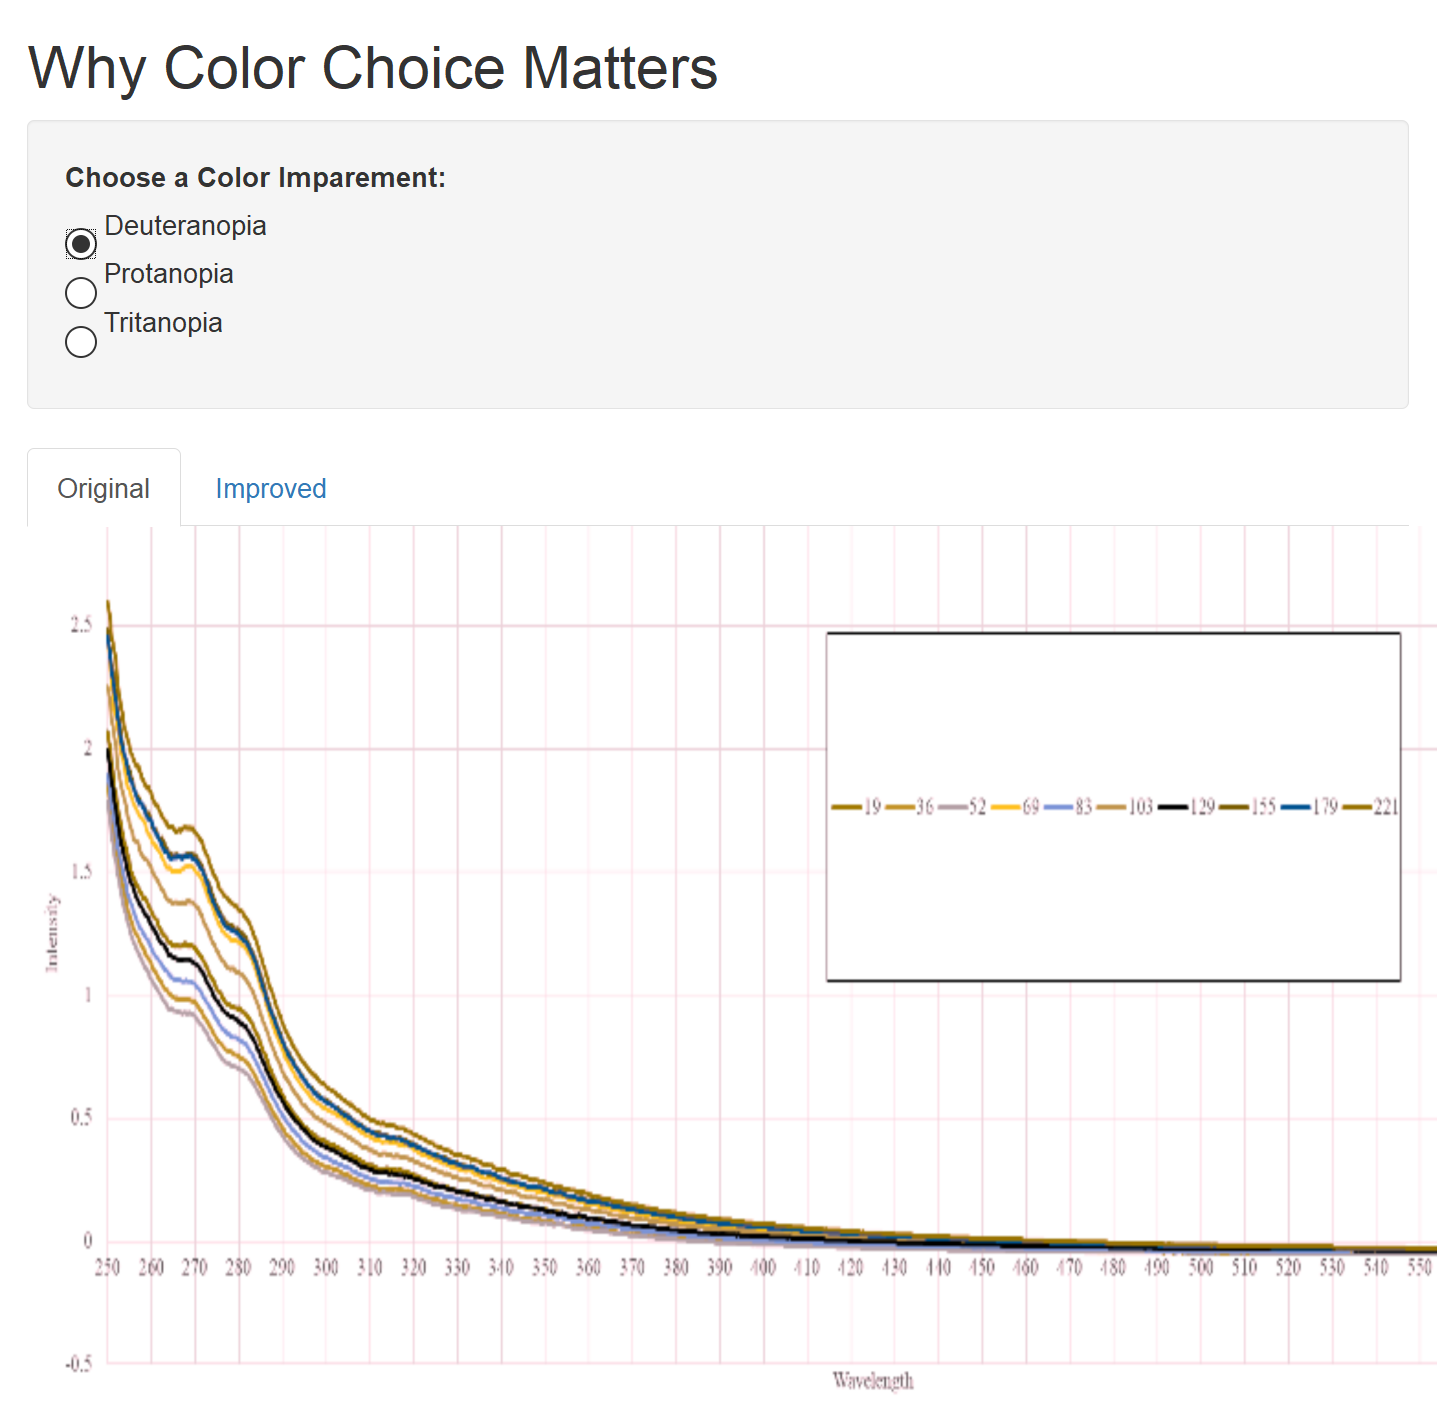
\includegraphics[width=.32\textwidth]{O_Deuteran.PNG} &
  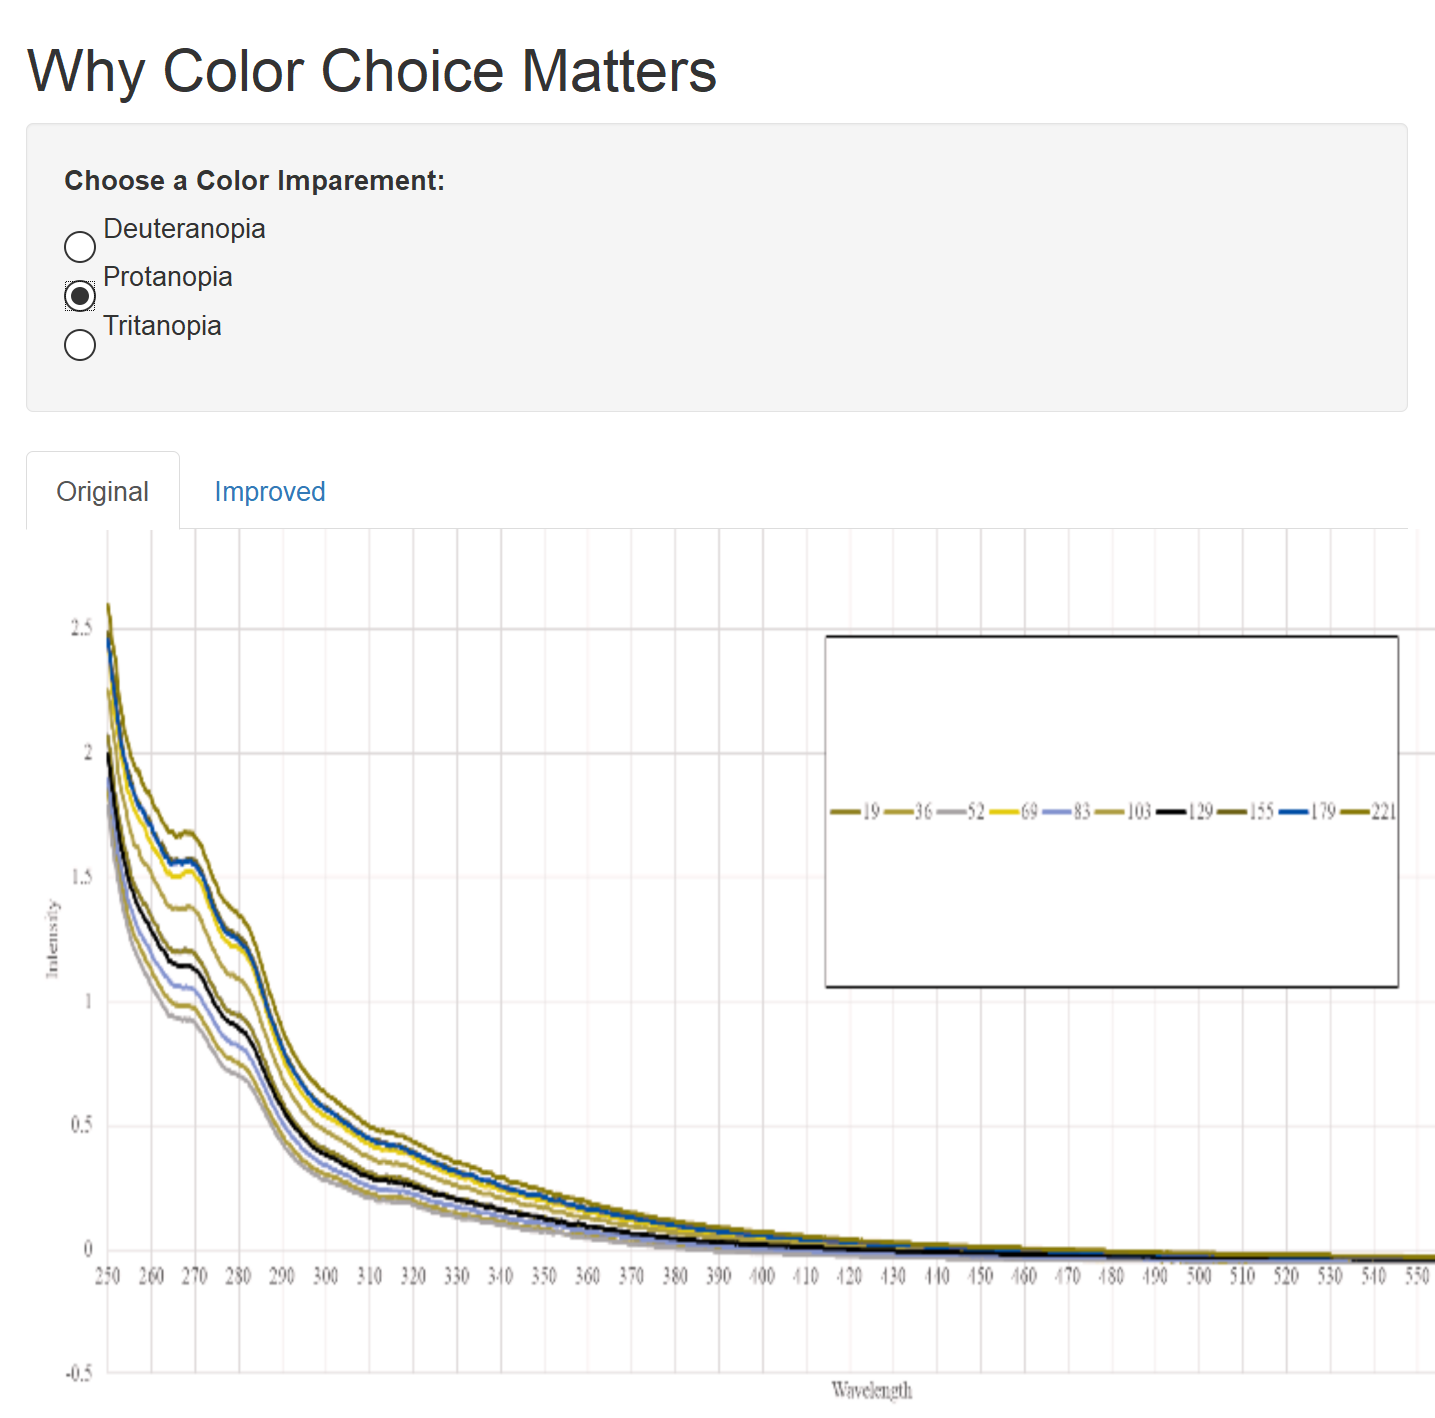
\includegraphics[width=.32\textwidth]{O_Protan.PNG} &
  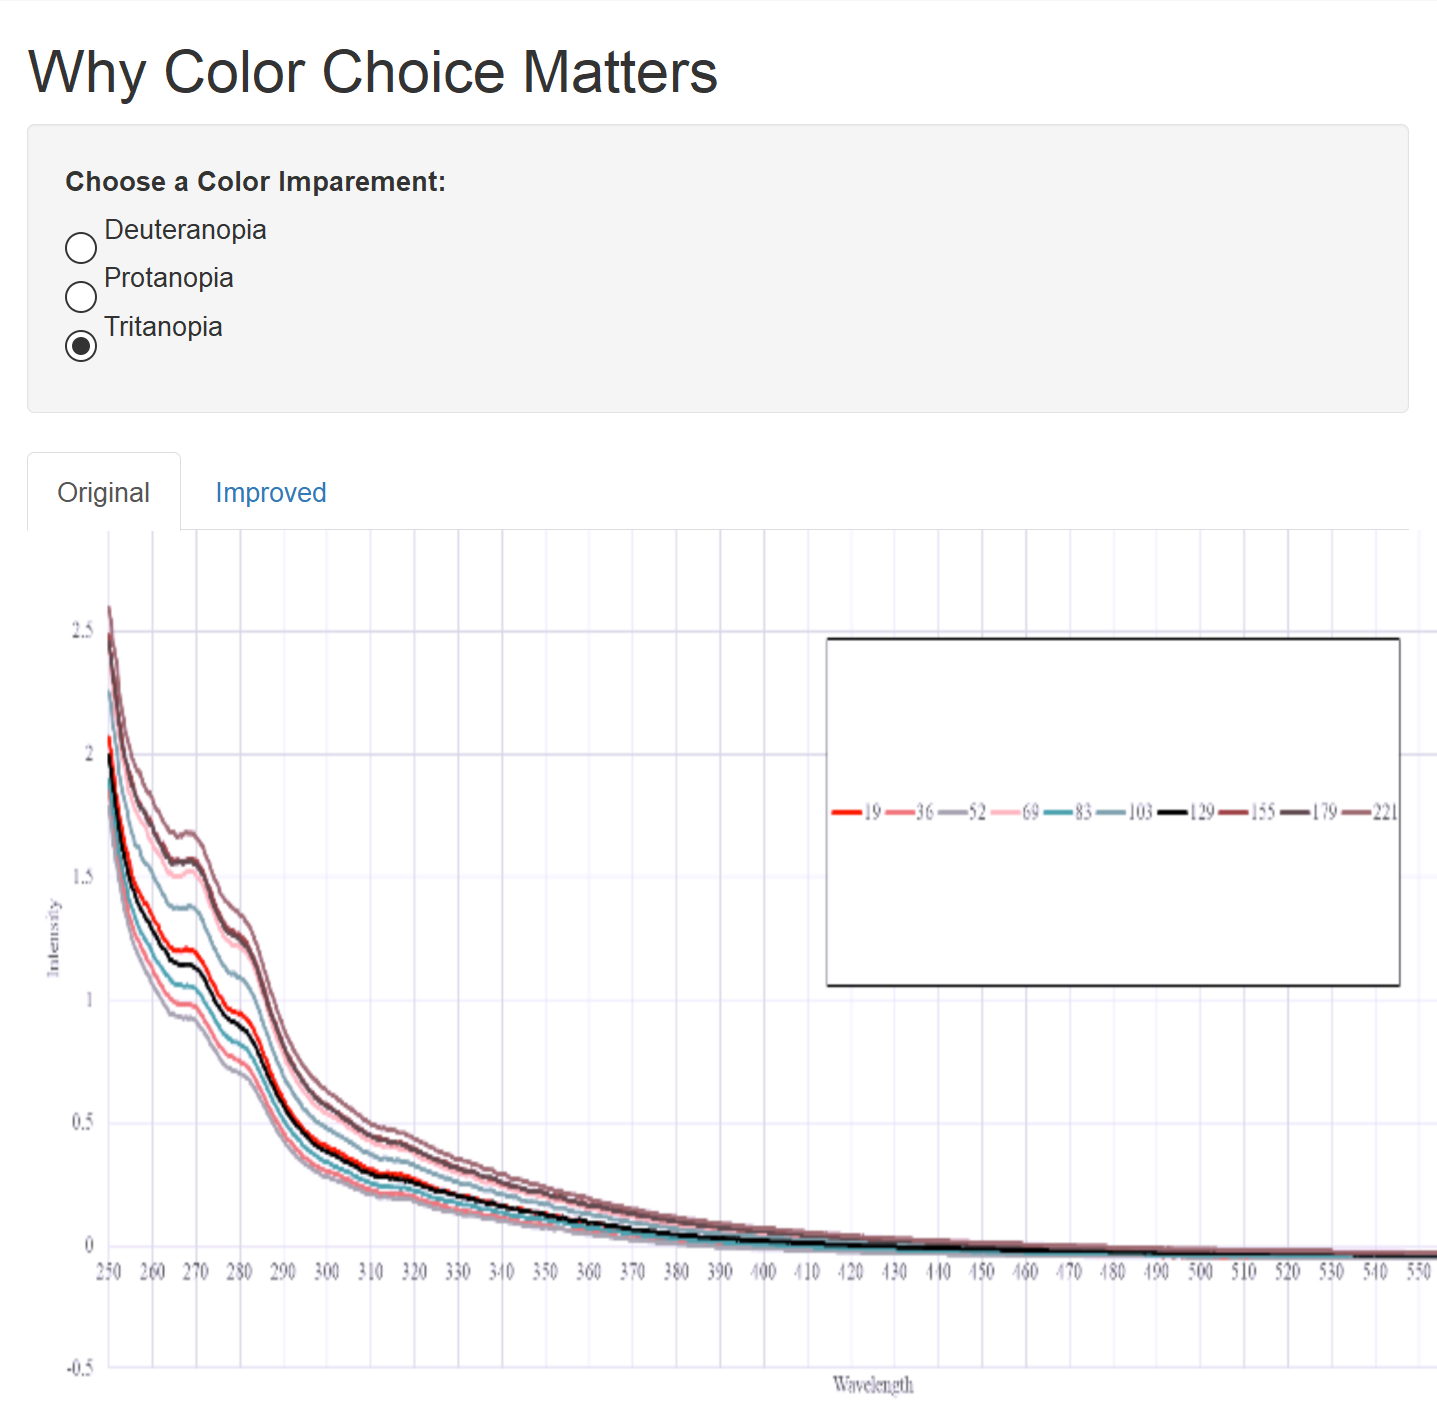
\includegraphics[width=.32\textwidth]{O_Tritan.PNG}\\
   & Improved & \\
  Protanopia & Deuteranopia & Tritanopia\\
  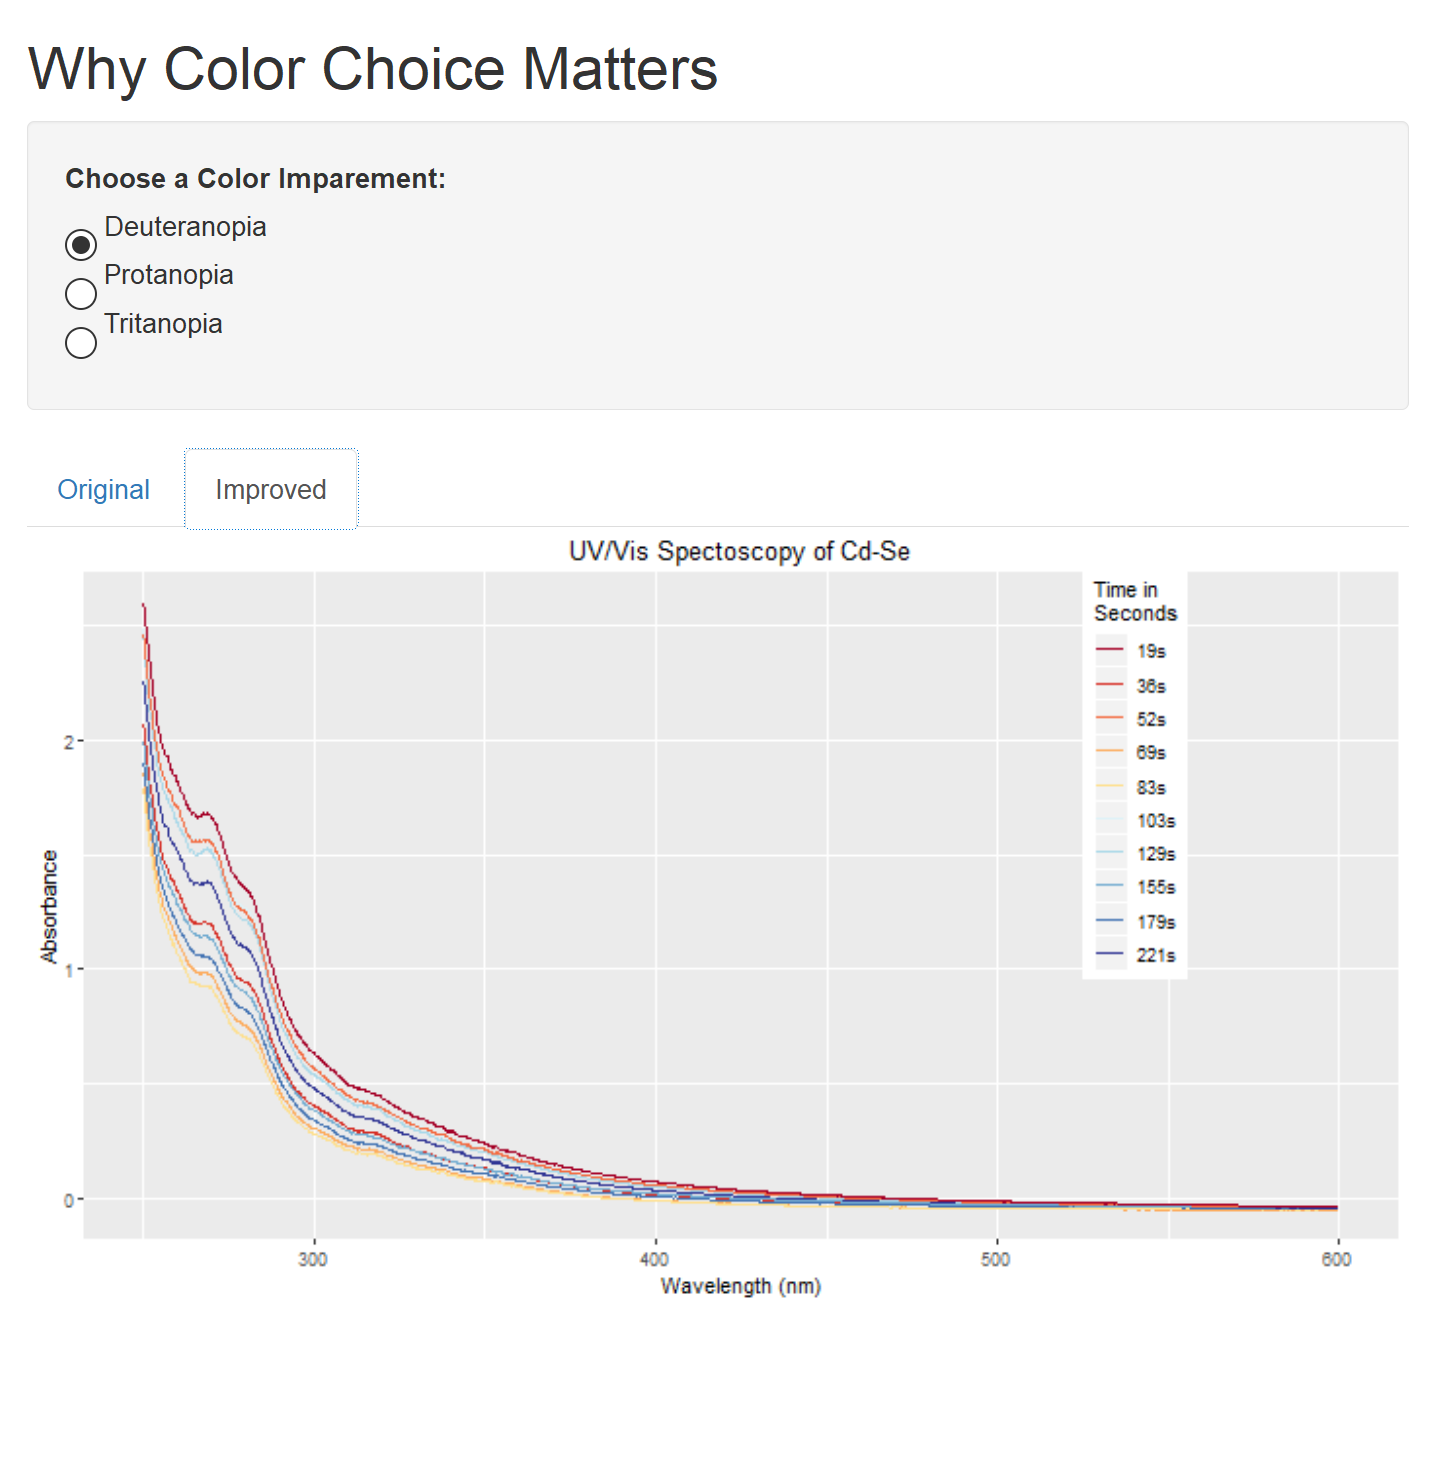
\includegraphics[width=.32\textwidth]{I_Deuteran.PNG} &
  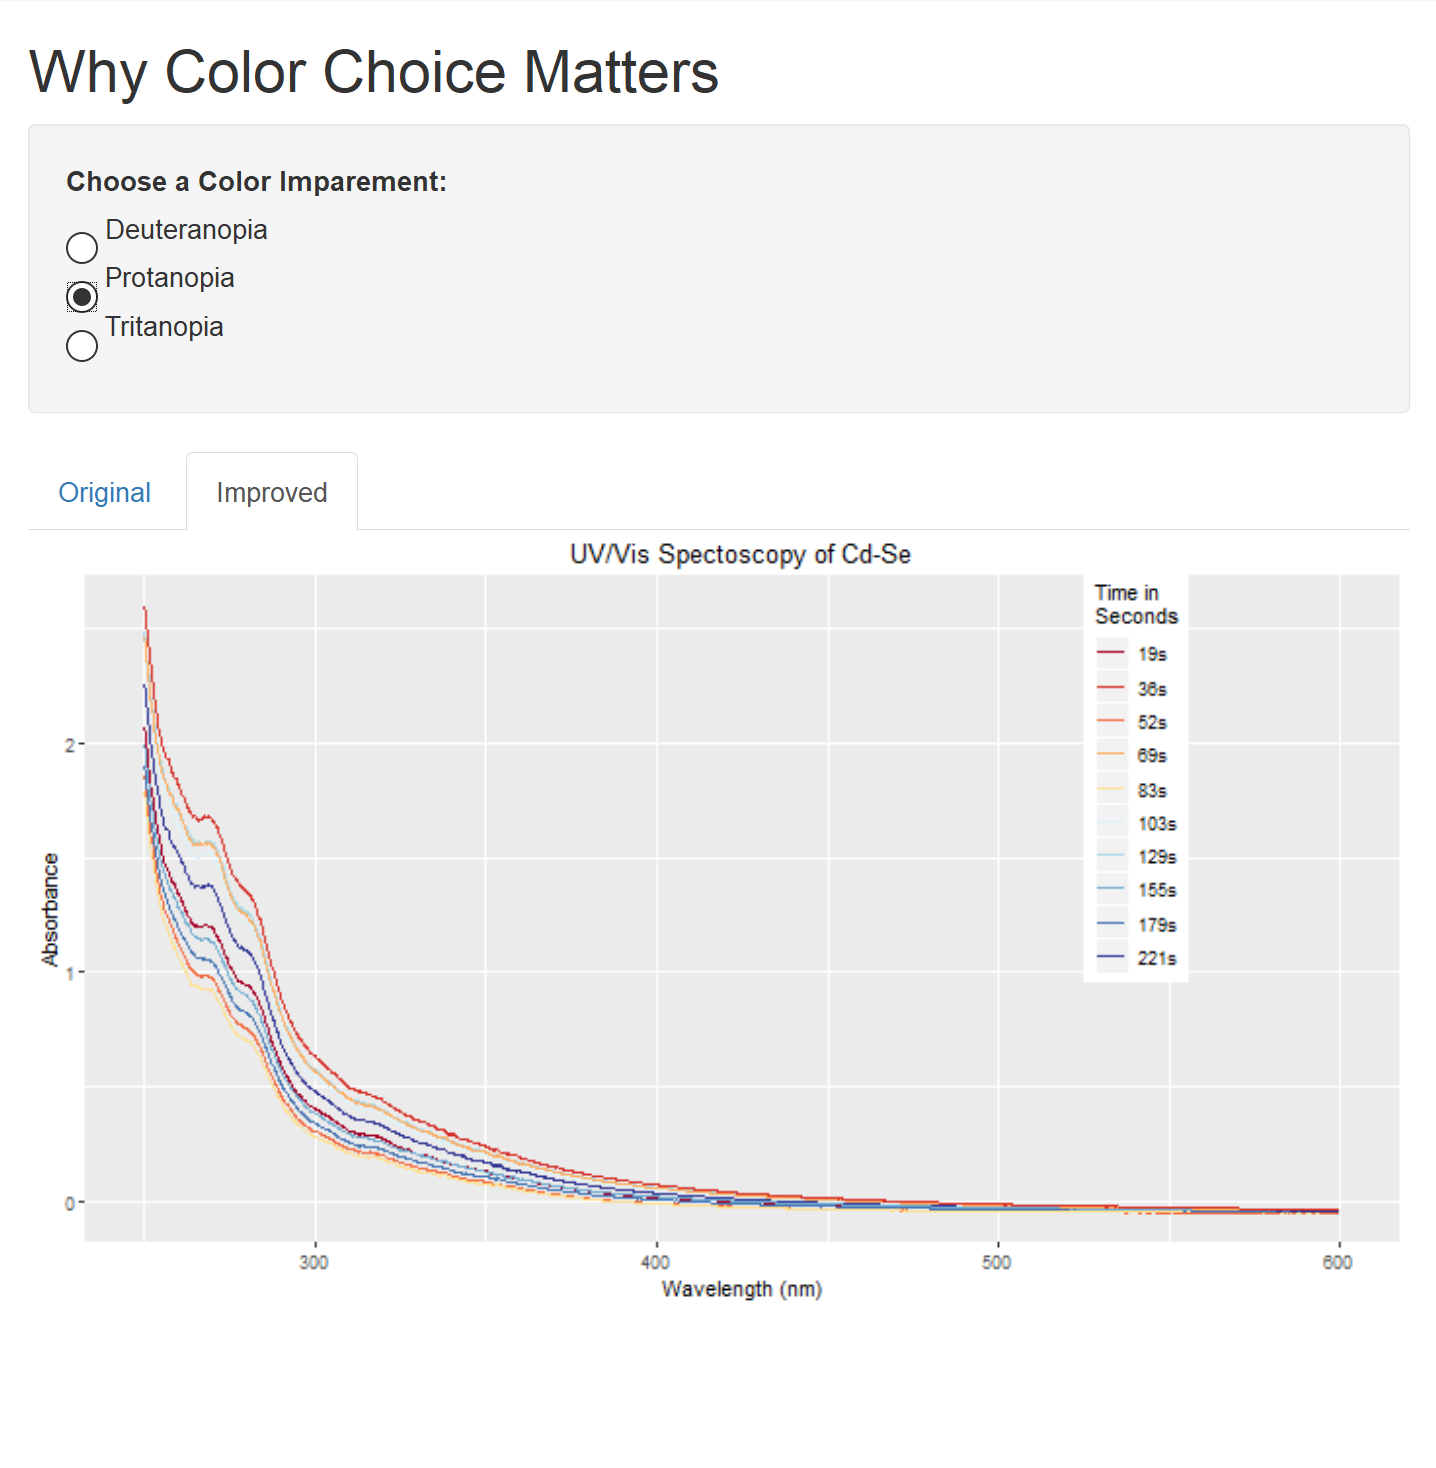
\includegraphics[width=.32\textwidth]{I_Protan.PNG} &
  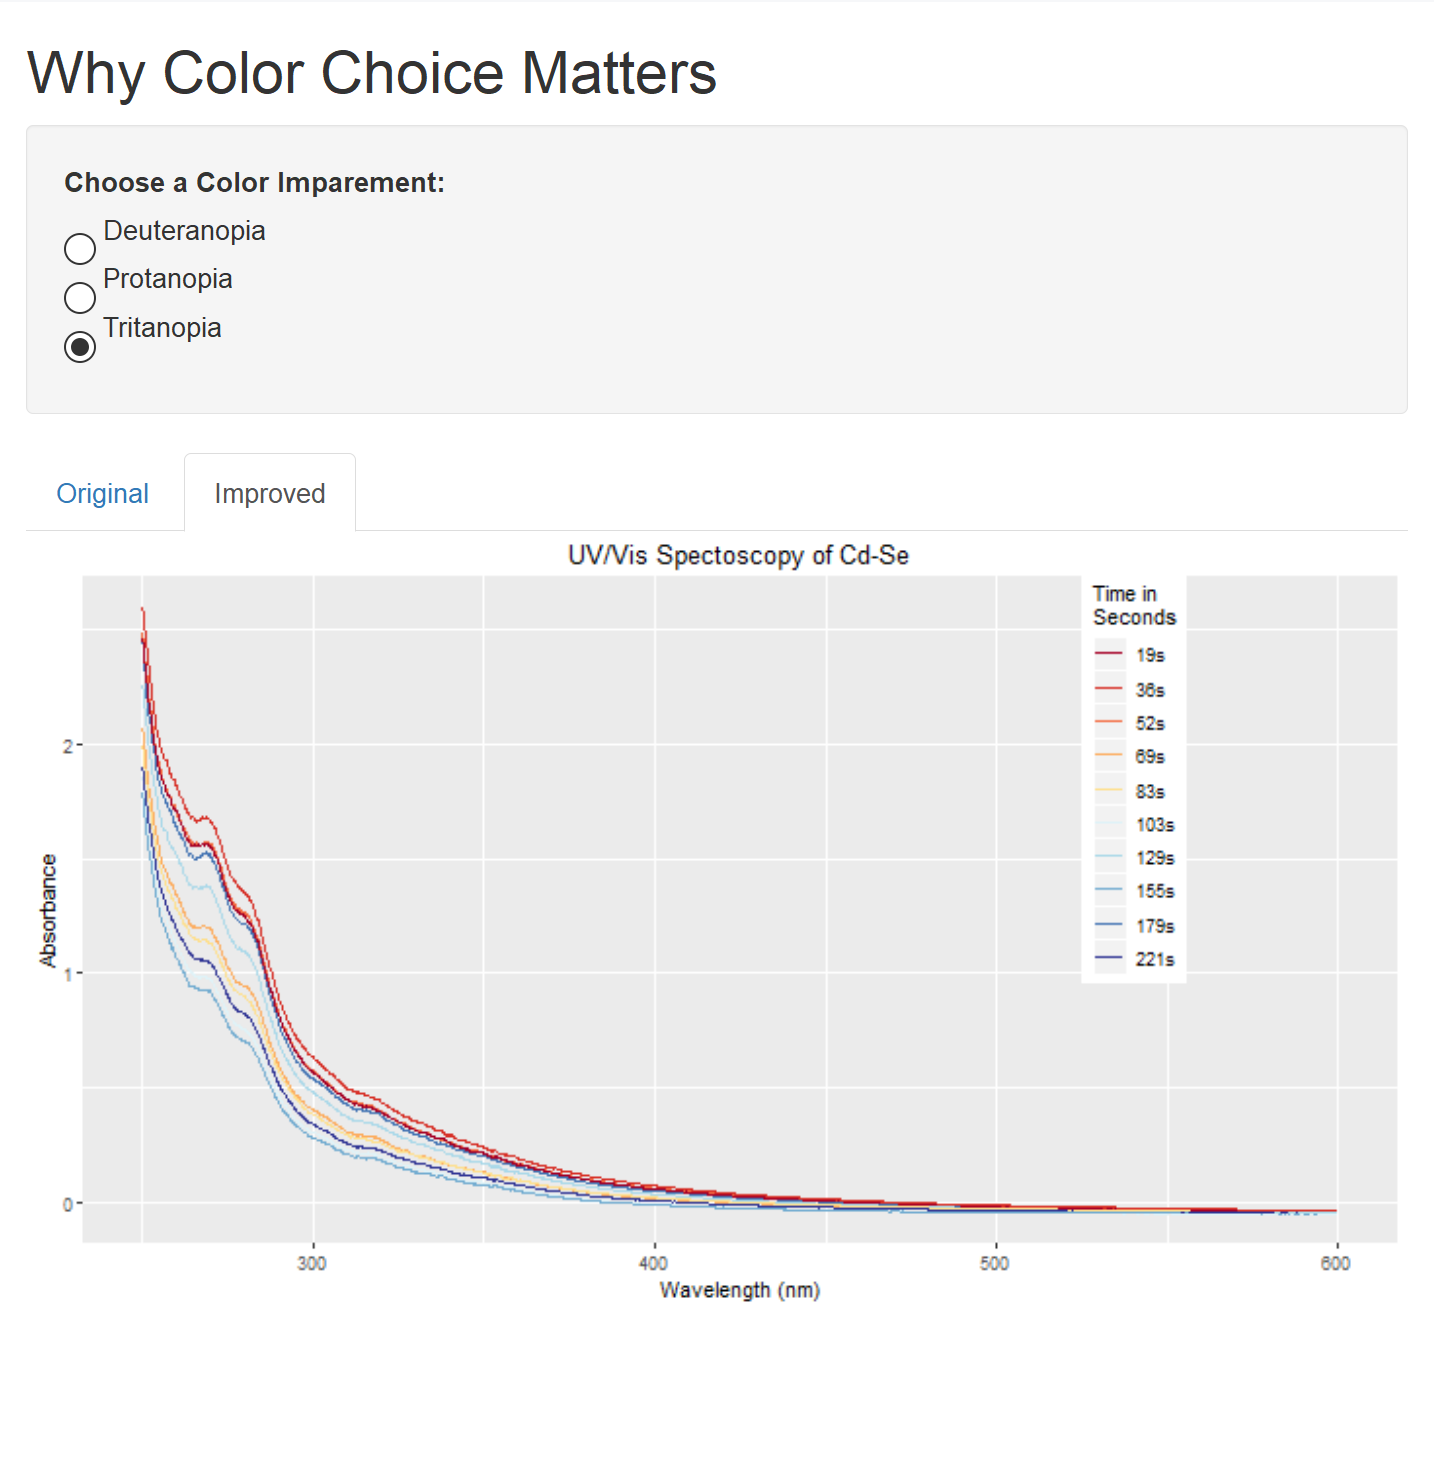
\includegraphics[width=.32\textwidth]{I_Tritan.PNG}\\
\end{array}$
\end{center}
\end{figure}

\newpage


\item {\bf Using the Grand Tour for an Interactive Clustering} (25 Points): \\
Load the file {\it hw03\_mystery.csv} into {\it GGobi}, the {\it rggobi} R package, or any other
standalone software or R package that allows you to apply a {\bf brush--tour} strategy
as introduced in the {\it Grand Tour} section of our lecture notes.

{\bf I have asked our computer support people
to install {\it GGobi}/{\it rggobi} on one or two publicly accessible computers in
our department. If you are interested in working on this question,
but do not have access to {\it GGobi}/{\it rggobi} on your own computer,
you will hopefully be able to use one of the computers here in
the department within the next few days. I will post an announcement in Canvas
when {\it GGobi}/{\it rggobi} have been installed on a 
departmental computer.}

My instructions below are written under the assumption that you are using {\it GGobi}.

For this question, you do not have to include any R code.


\begin{enumerate}

\item (5 Points)
Start the grand tour and select the six variables called {\it V1, $\ldots$, V6}.
Do {\bf not} select the variable {\it Row}. In the grand tour window,
select {\it Options $\rightarrow$ Show Axes} to show the projection of the
variable axes. Adjust the speed of the tour as desired. 

First look for obvious outliers
in the grand tour. These are single points that behave rather differently from all
other points in the tour. Once you have spotted an outlier, stop the tour
and brush this point with a big red $X$. Continue and find the next outlier, etc.
There are $\geq 1$ and $\leq 5$ outliers. How many outliers did you find?

Continue the tour and find a projection where
all of your outliers are visible and well separated from the
other data points at the same time. Such a projection exists.
Do some fine adjustment of this projection with the mouse. Which 
variables contribute most to this projection? Also include a screenshot
(or photo taken with your phone) of this projection
as part of your answer. Make sure that the variable axes are visible. 

{\scriptsize
  I noticed {\bf 4} total outliers that seemed reasonably significant to me.  In the screenshot below, {\it V3} contributes the most, followed by {\it V6} and {\it V1}.
  \begin{center}
  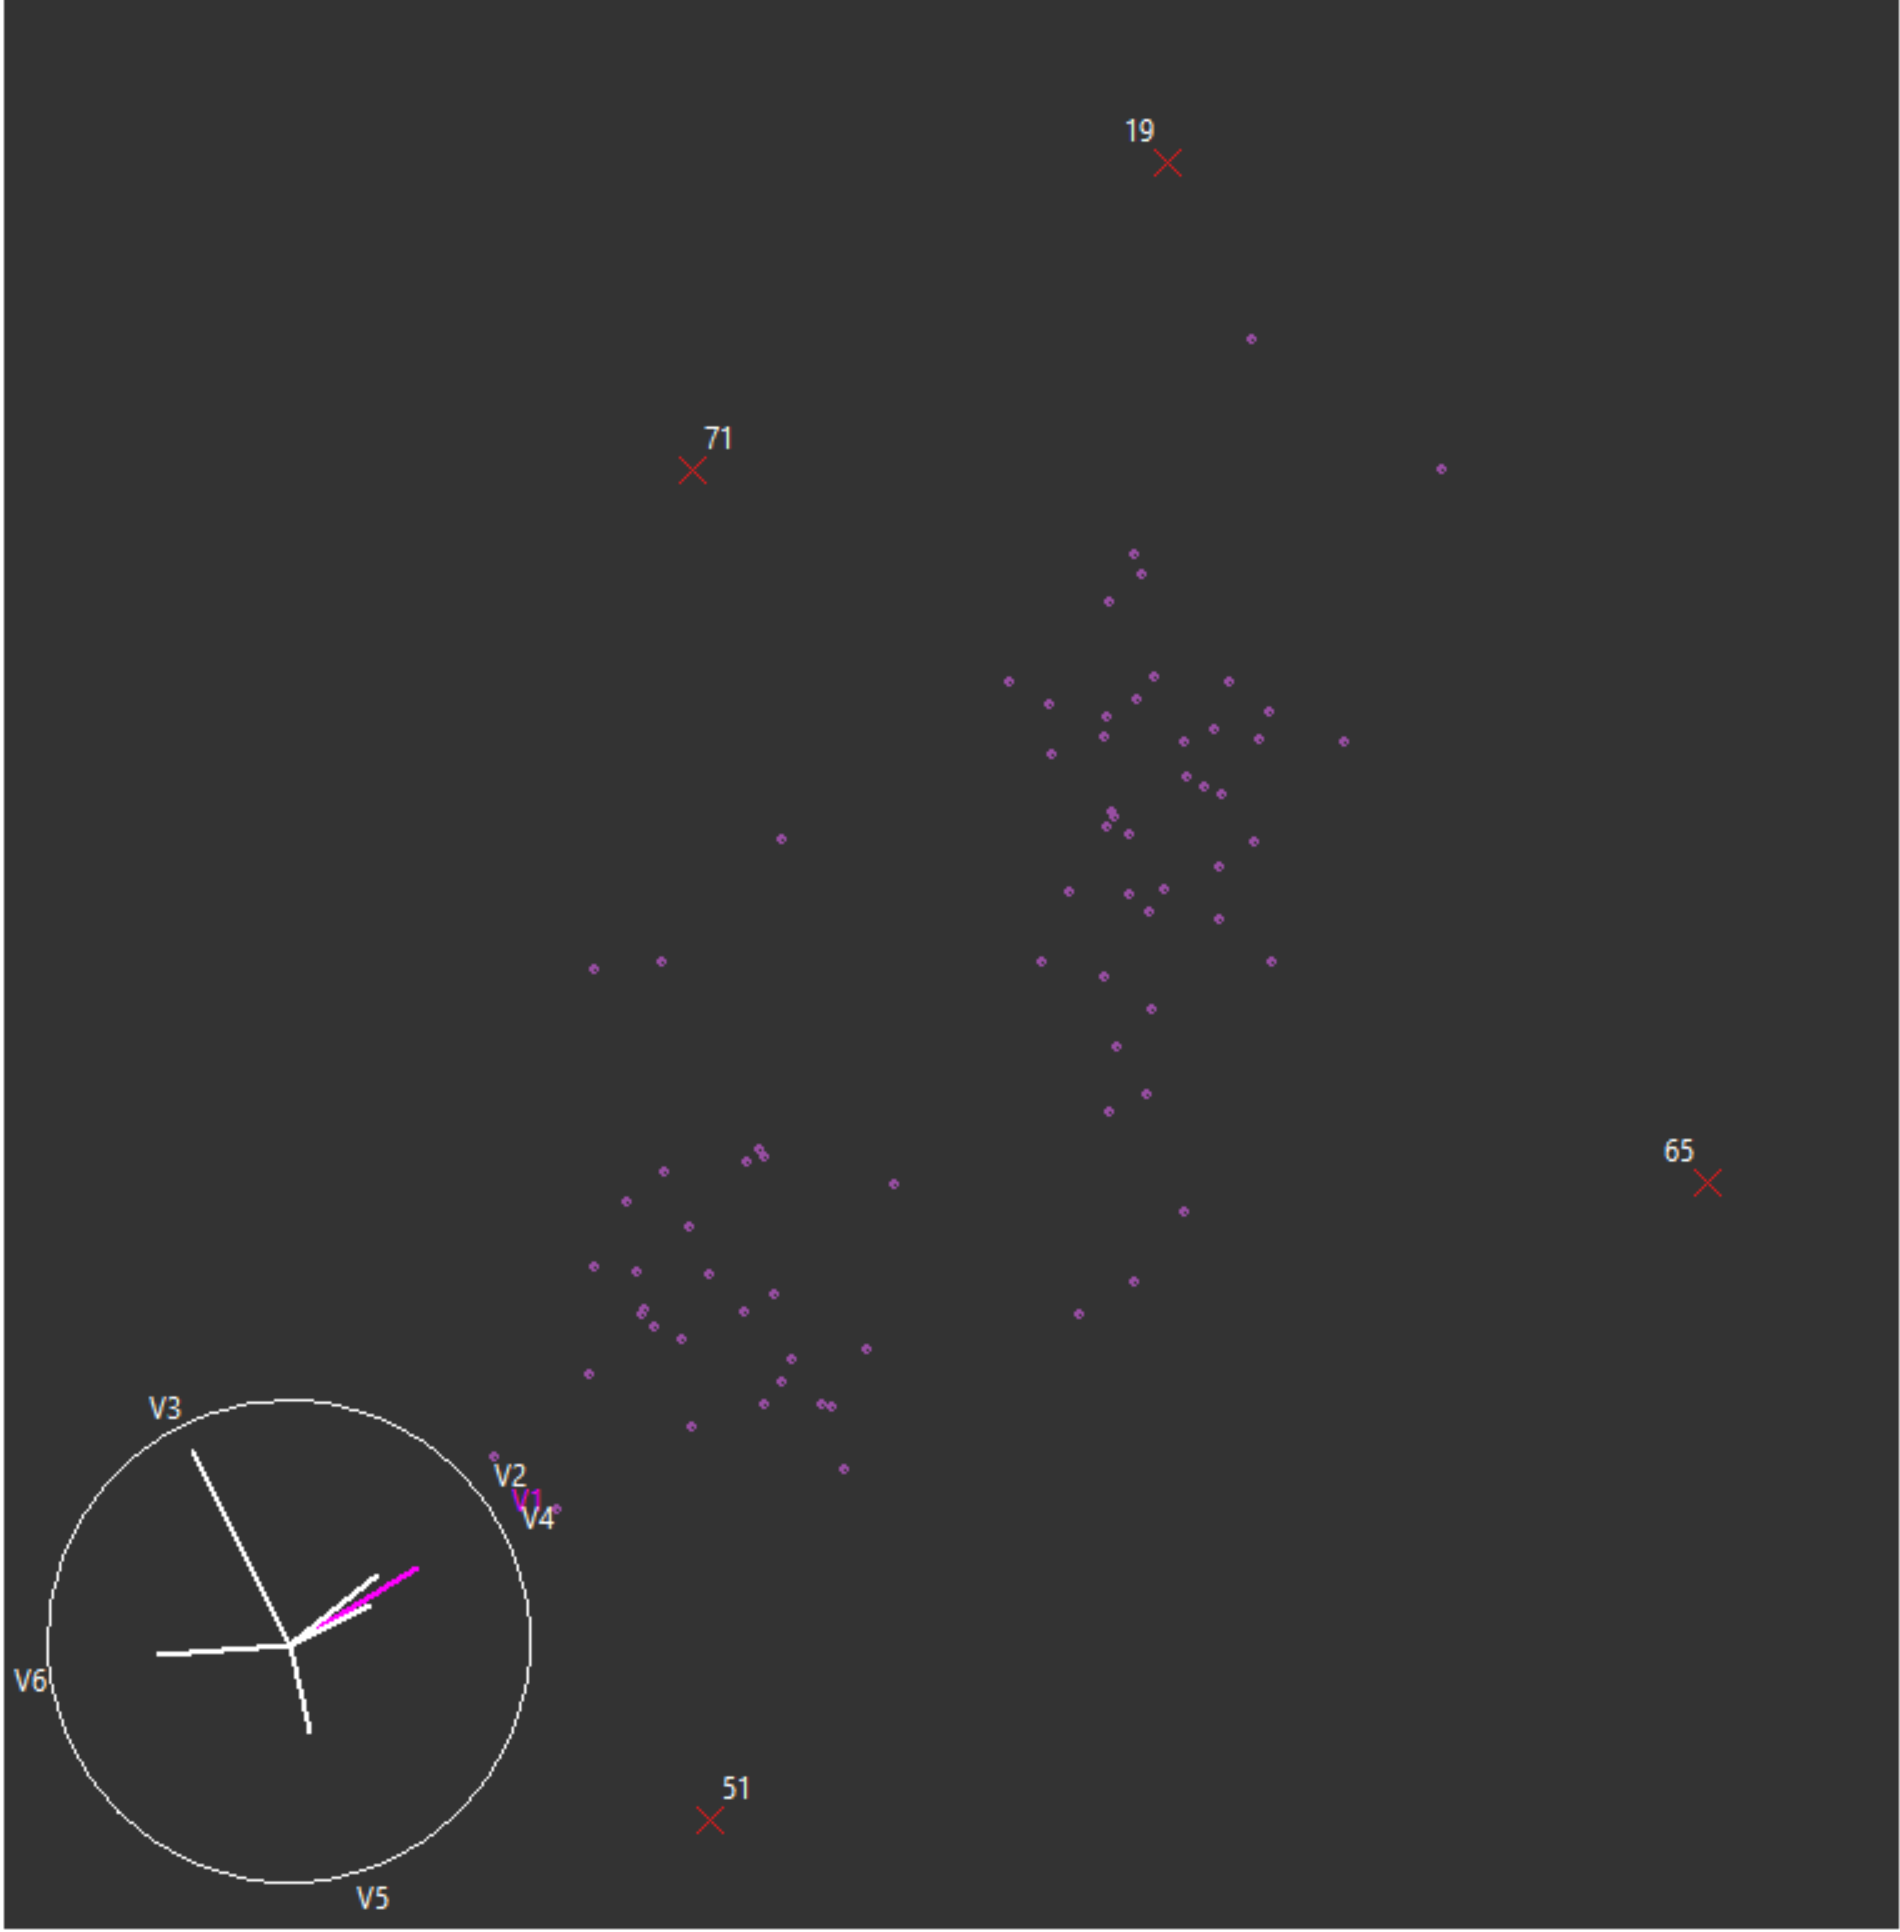
\includegraphics[width=9.5 cm]{p4a.png}
\end{center}
}


\item (4 Points)
Now focus on clusters via the grand tour. There are $\geq 2$ and $\leq 5$
clusters in this data set. Whenever you think you identified a cluster,
i.e., a group of points that moves in a different direction, persistently
brush it with a new color and symbol. 

If you paused the tour a fraction of a second too late, do some adjustment
of the projection with the mouse to get back to a more interesting projection.
Do not brush your previously detected
outliers again! 

After each new cluster you detected, take a screenshot (or photo)
and include it as part of your answer. As before, make sure that the 
variable axes are visible. How many main clusters did you detect? 

{\scriptsize
  I identified {\bf 3} distinct clusters.  I've attached two screenshots in the order I identified the groupings below:.
  \begin{center}
    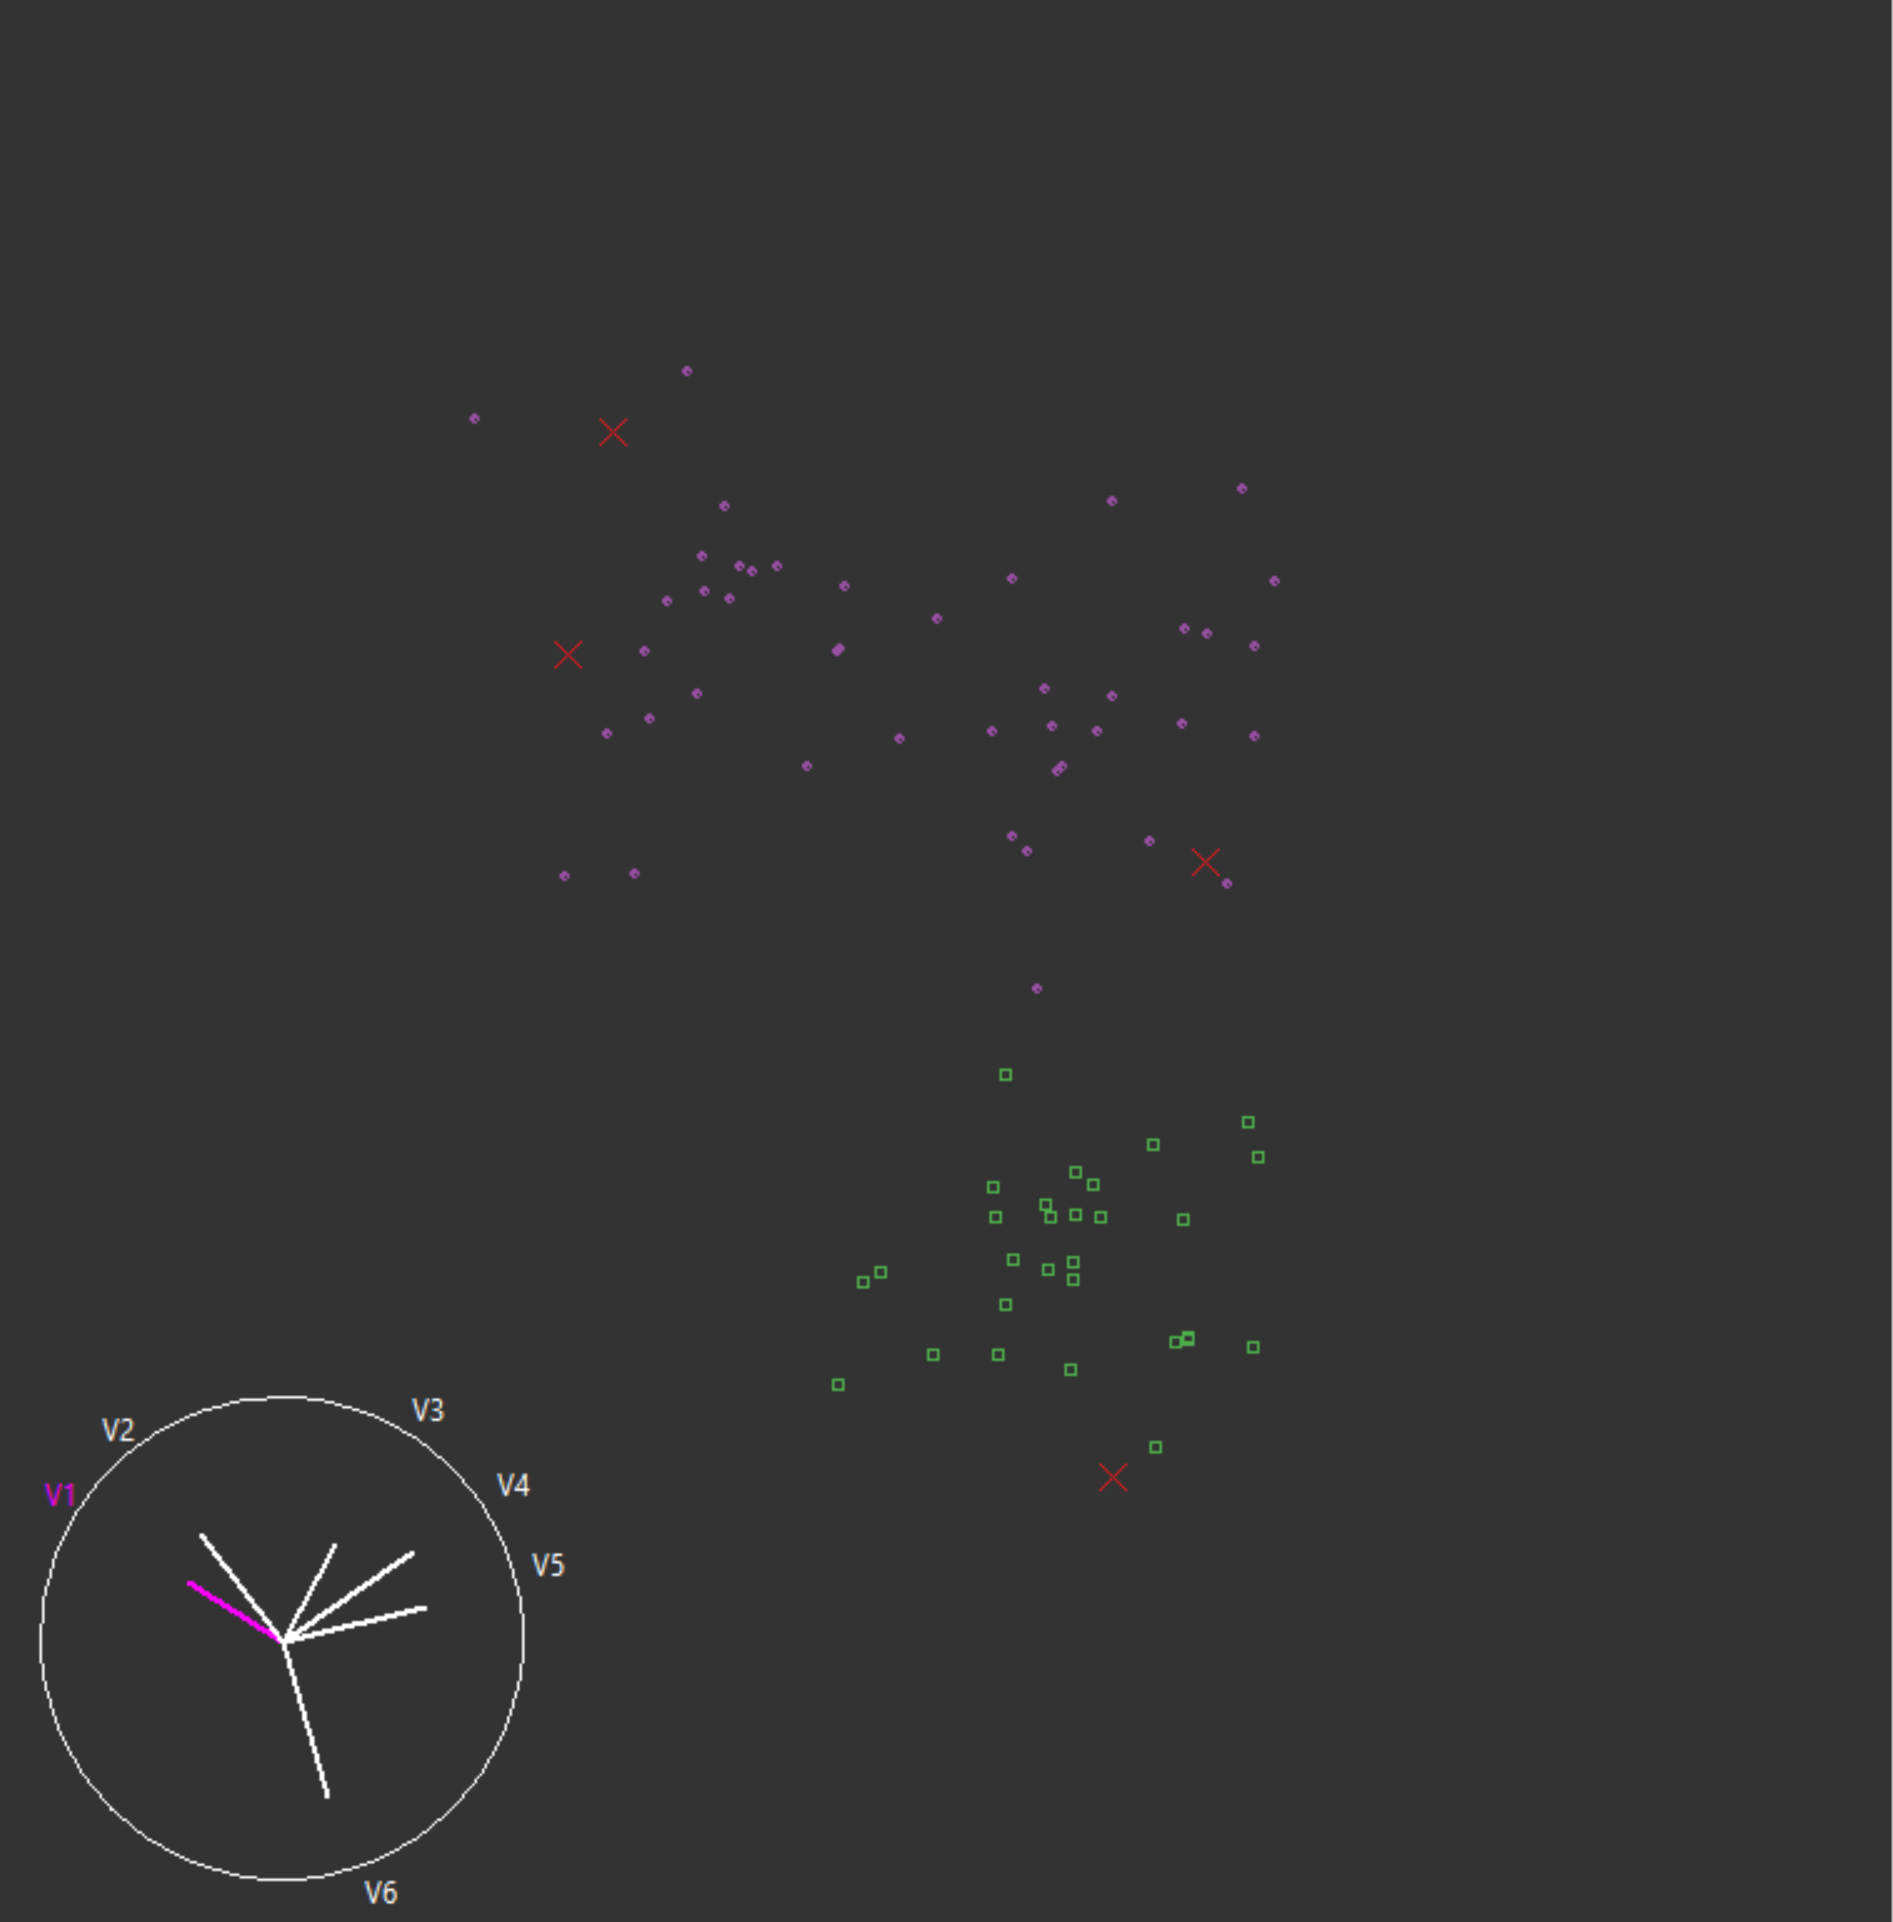
\includegraphics[width=6.5 cm]{p4bi.png}
    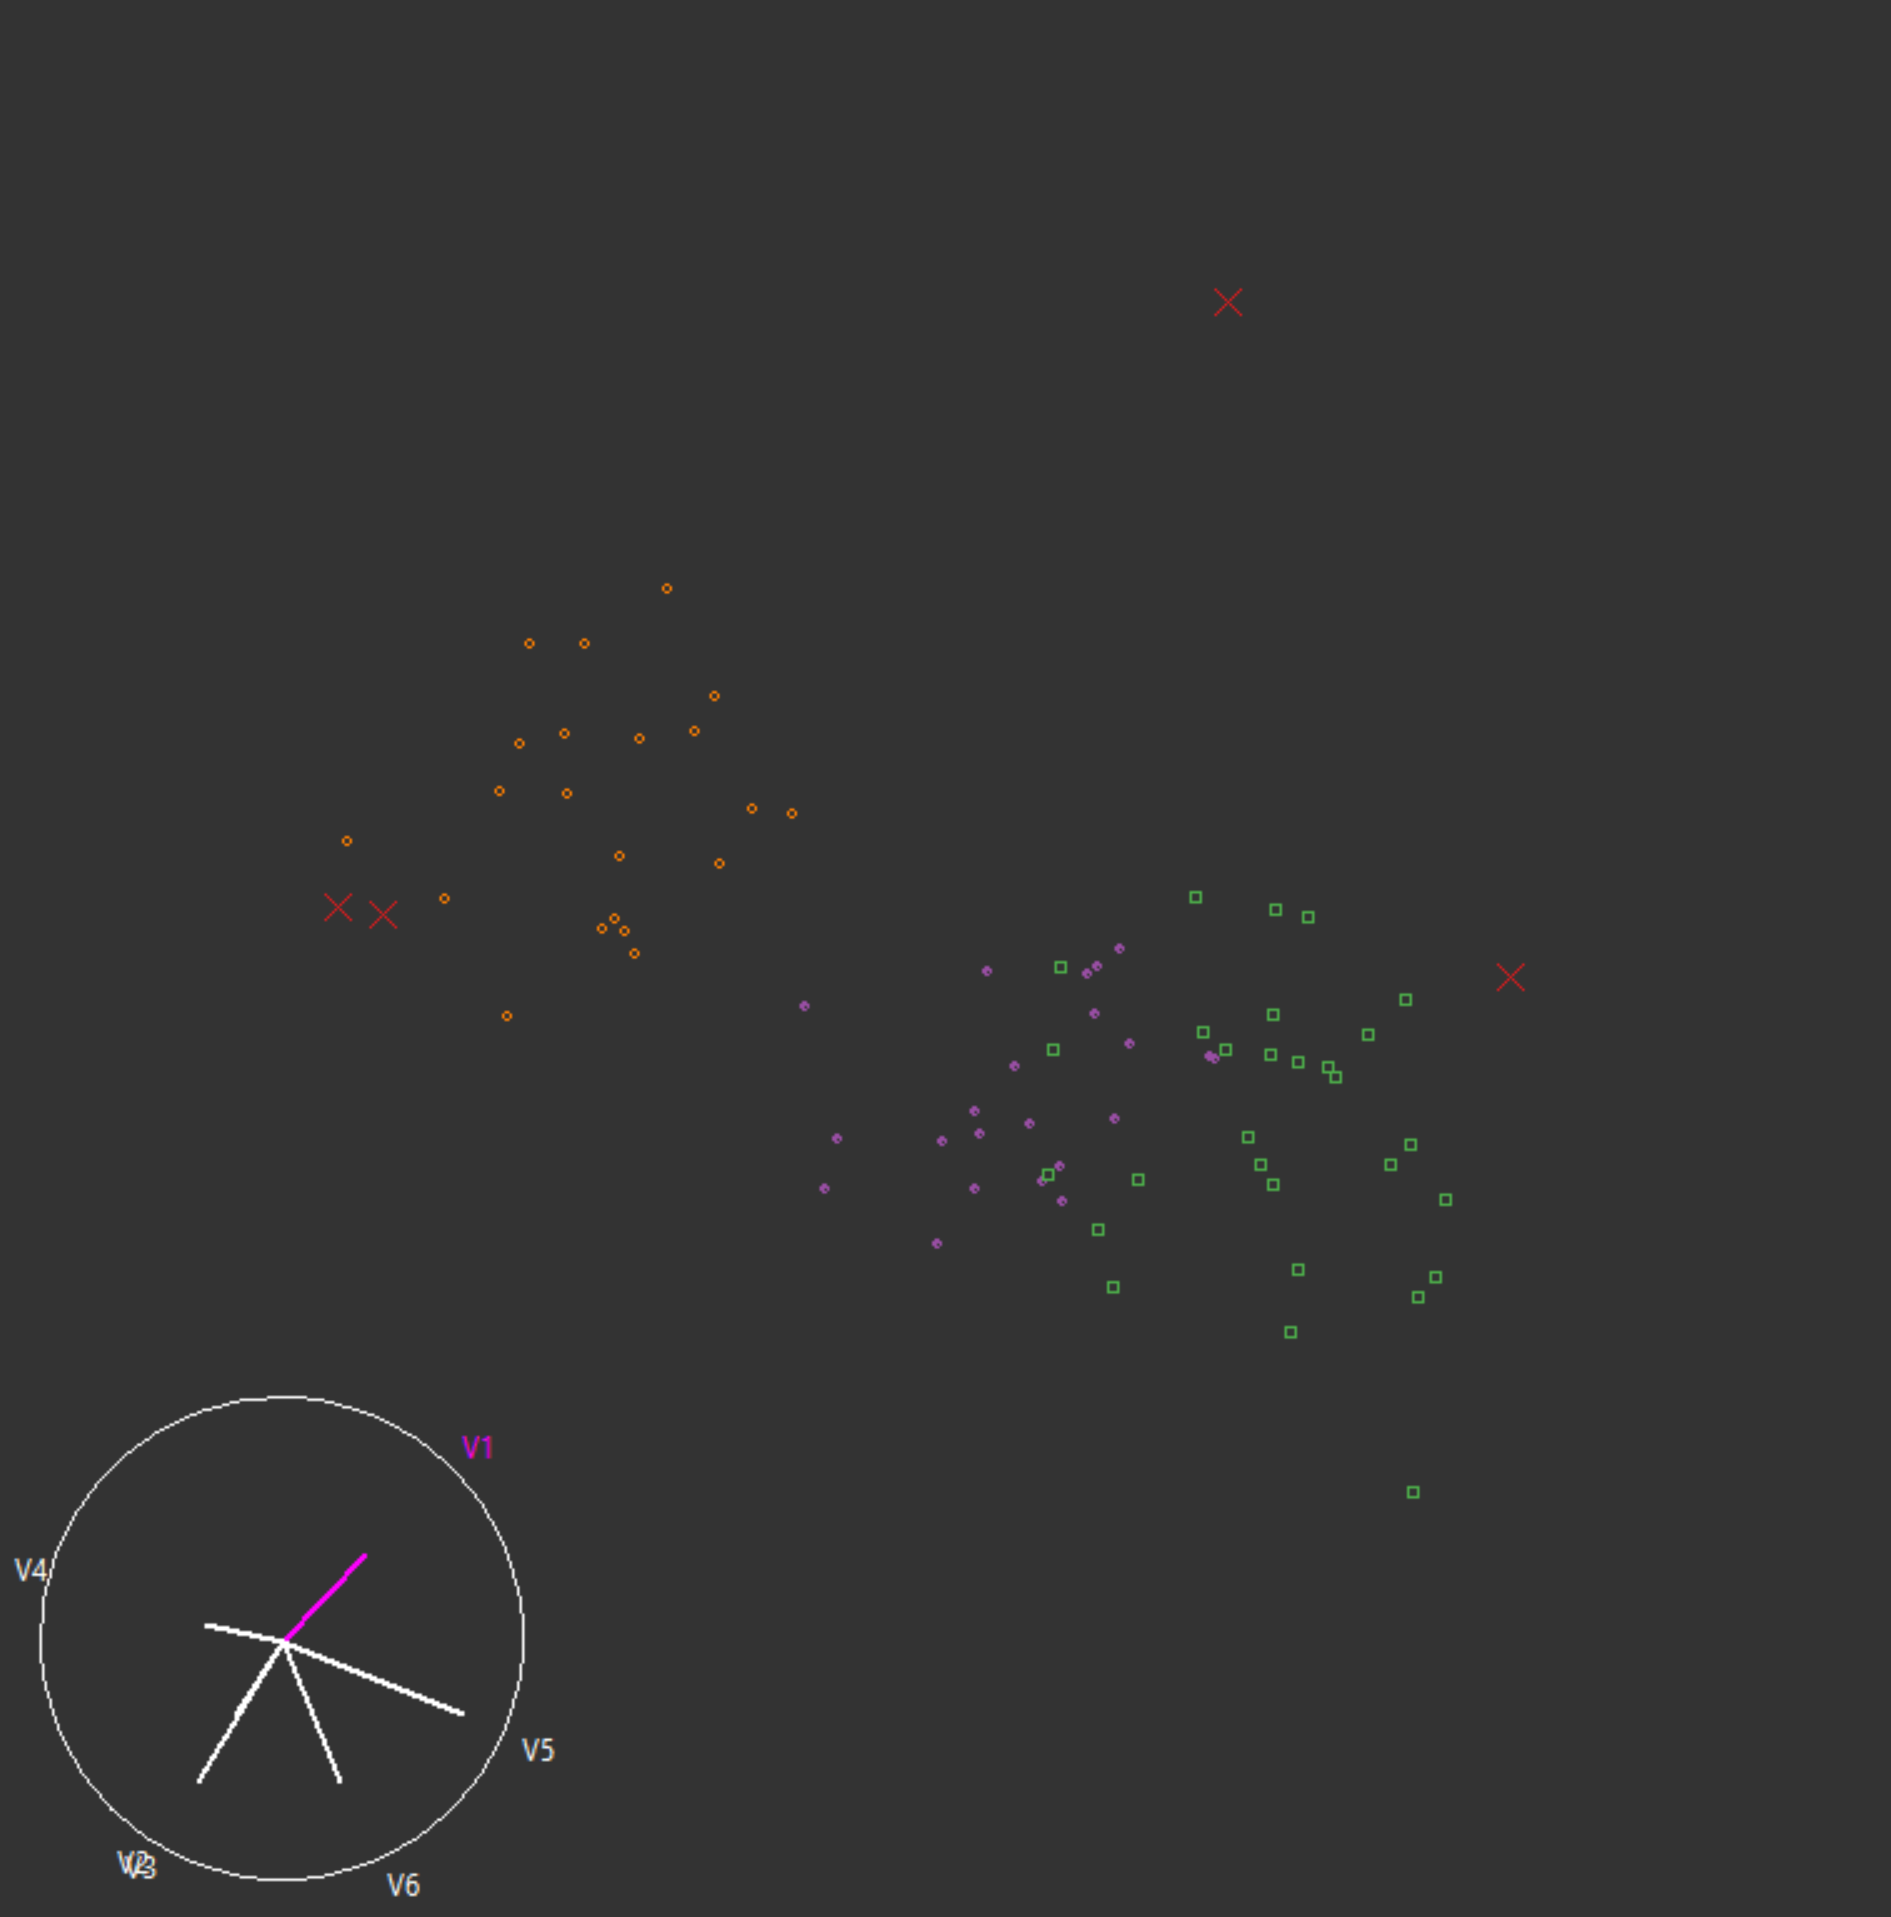
\includegraphics[width=6.5 cm]{p4bii.png}\\
  \end{center}
}

\item (4 Points)
Find a projection in the grand tour that separates your clusters and
the outliers reasonably well. There may not be a perfect projection
that separates all clusters and the outliers at the same time.

Also activate a parallel coordinate plot (PCP) and a scatterplot matrix of all
six variables and {\it Row}. Make sure that the variables
appear in the order {\it V1, $\ldots$, V6, Row}. If this is not the case
pull the axes in the PCP until they appear in the right place in {\it GGobi}.
For the scatterplot matrix, unselect variables and select them in the
proper order again in {\it GGobi}. Include a screenshot of the final projection
from the grand tour, the PCP, and the scatterplot matrix.
  \begin{center}
    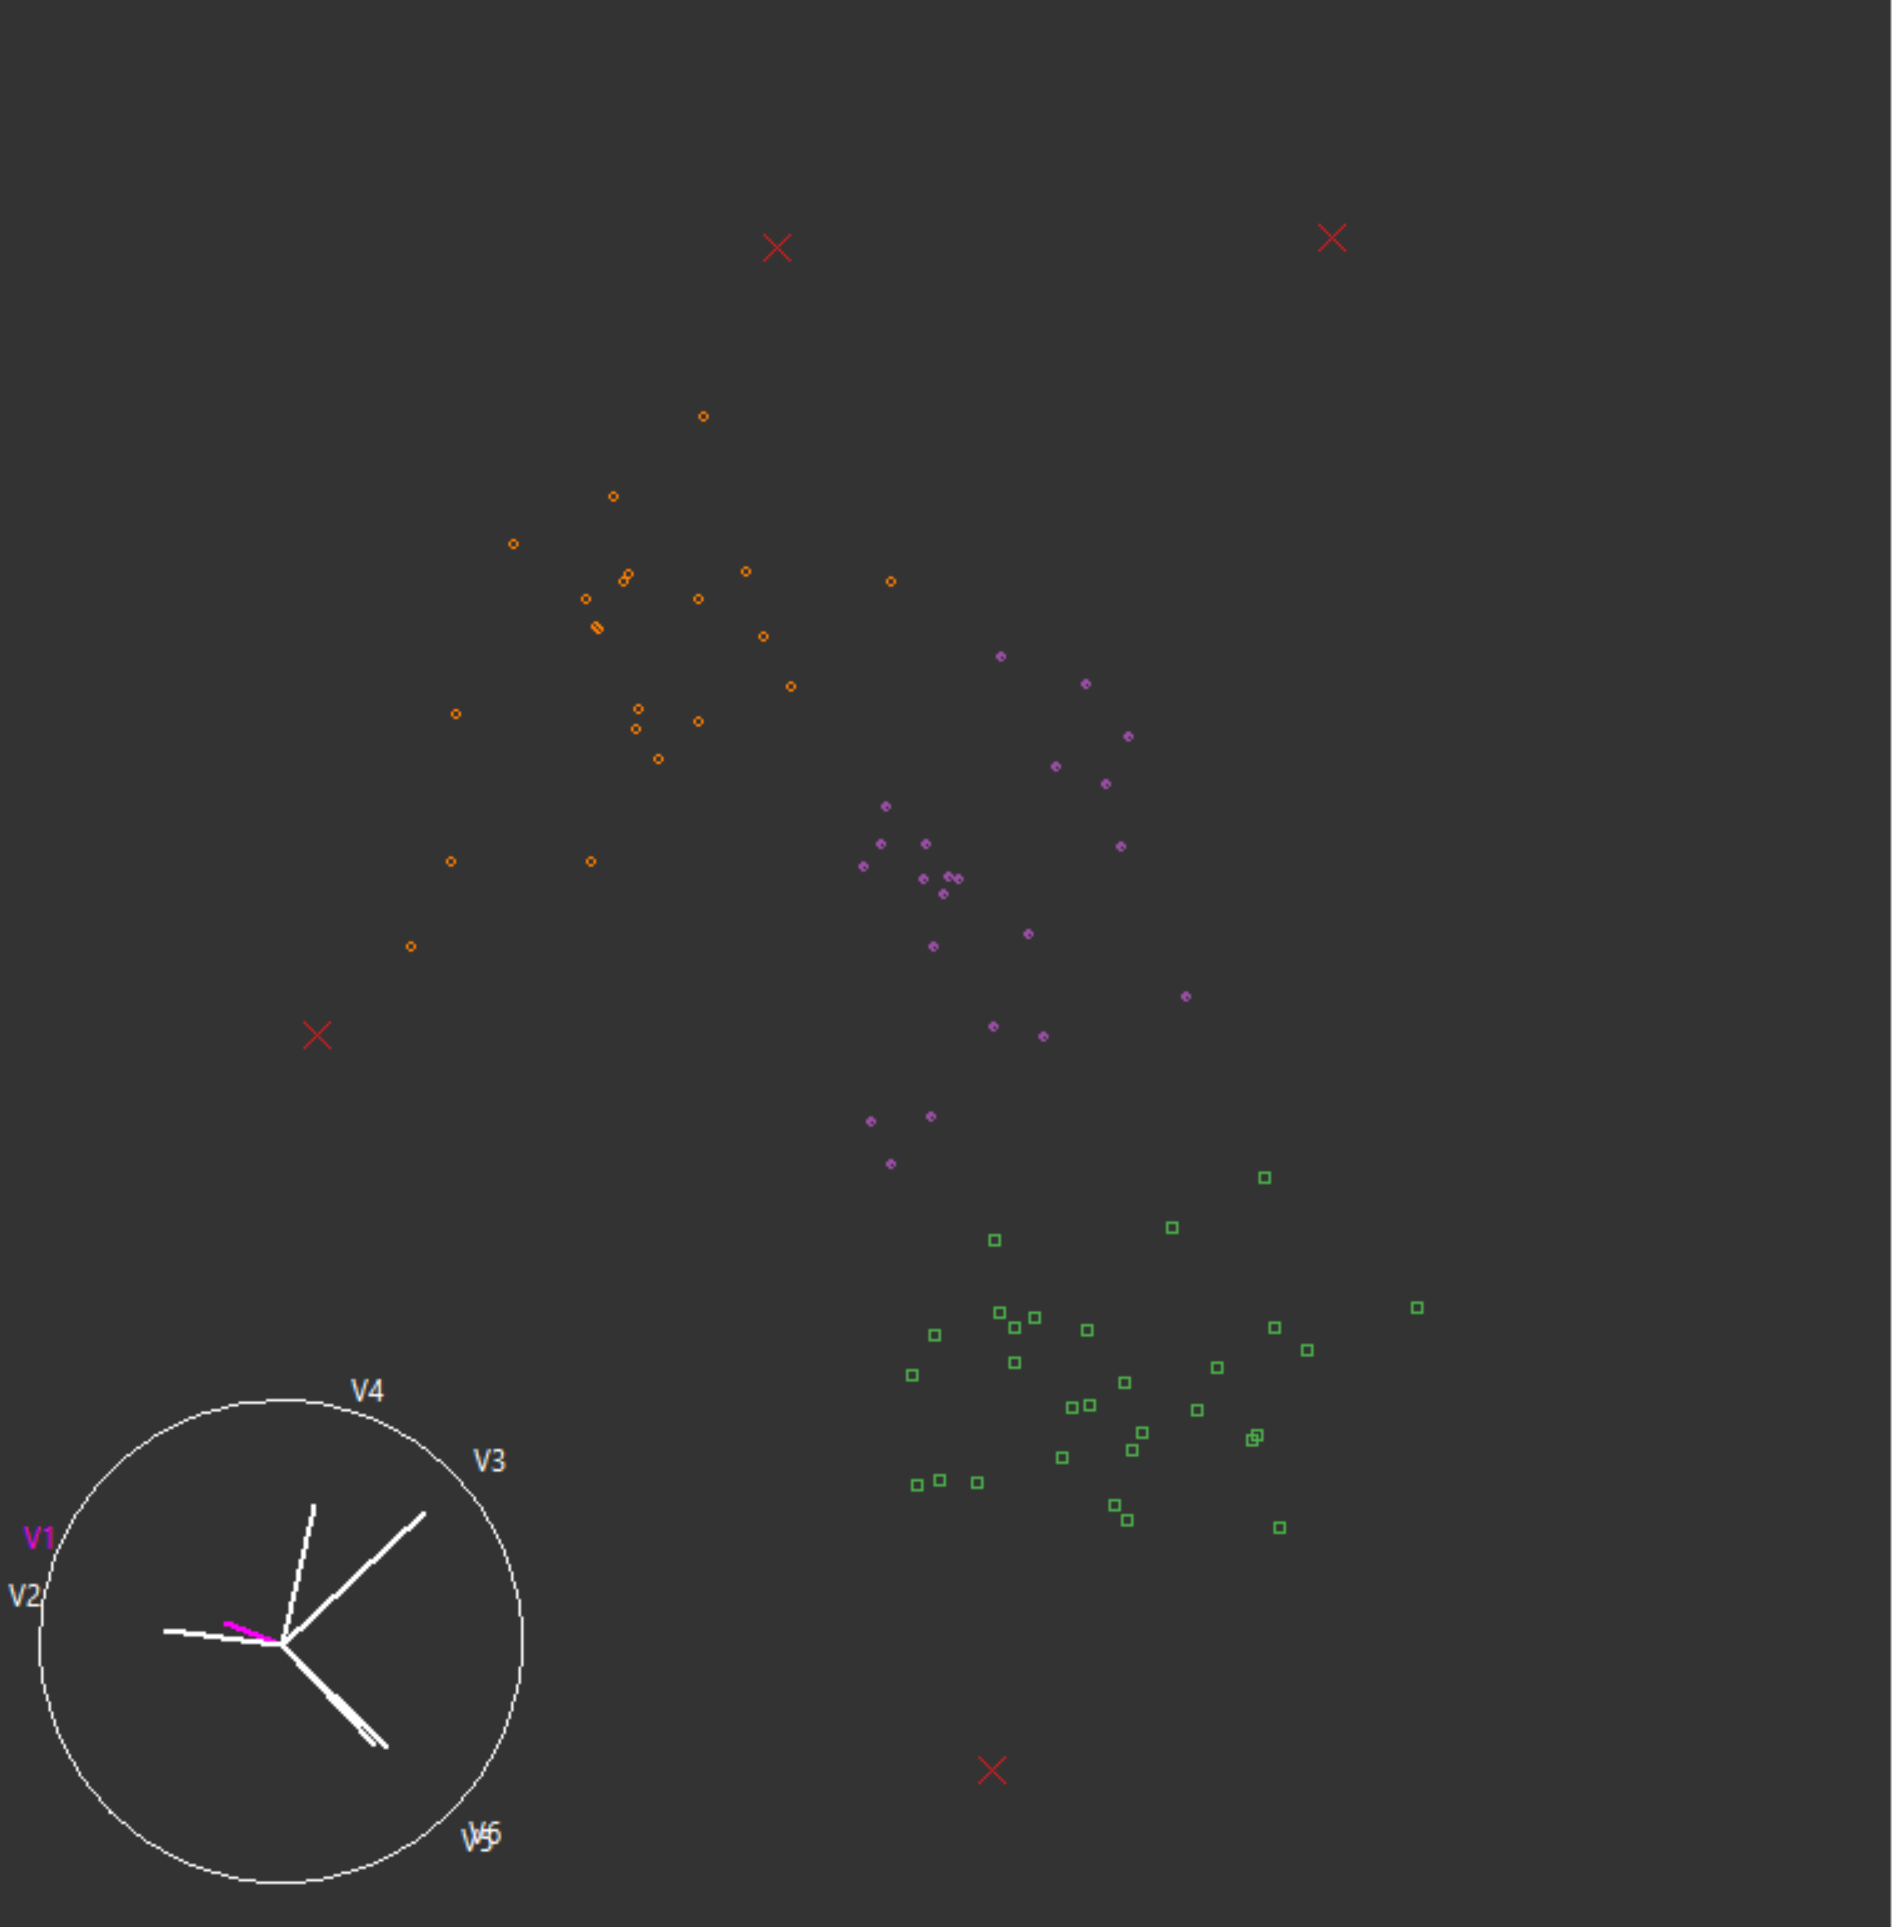
\includegraphics[width=11 cm]{p4c_Tour.png}\\
    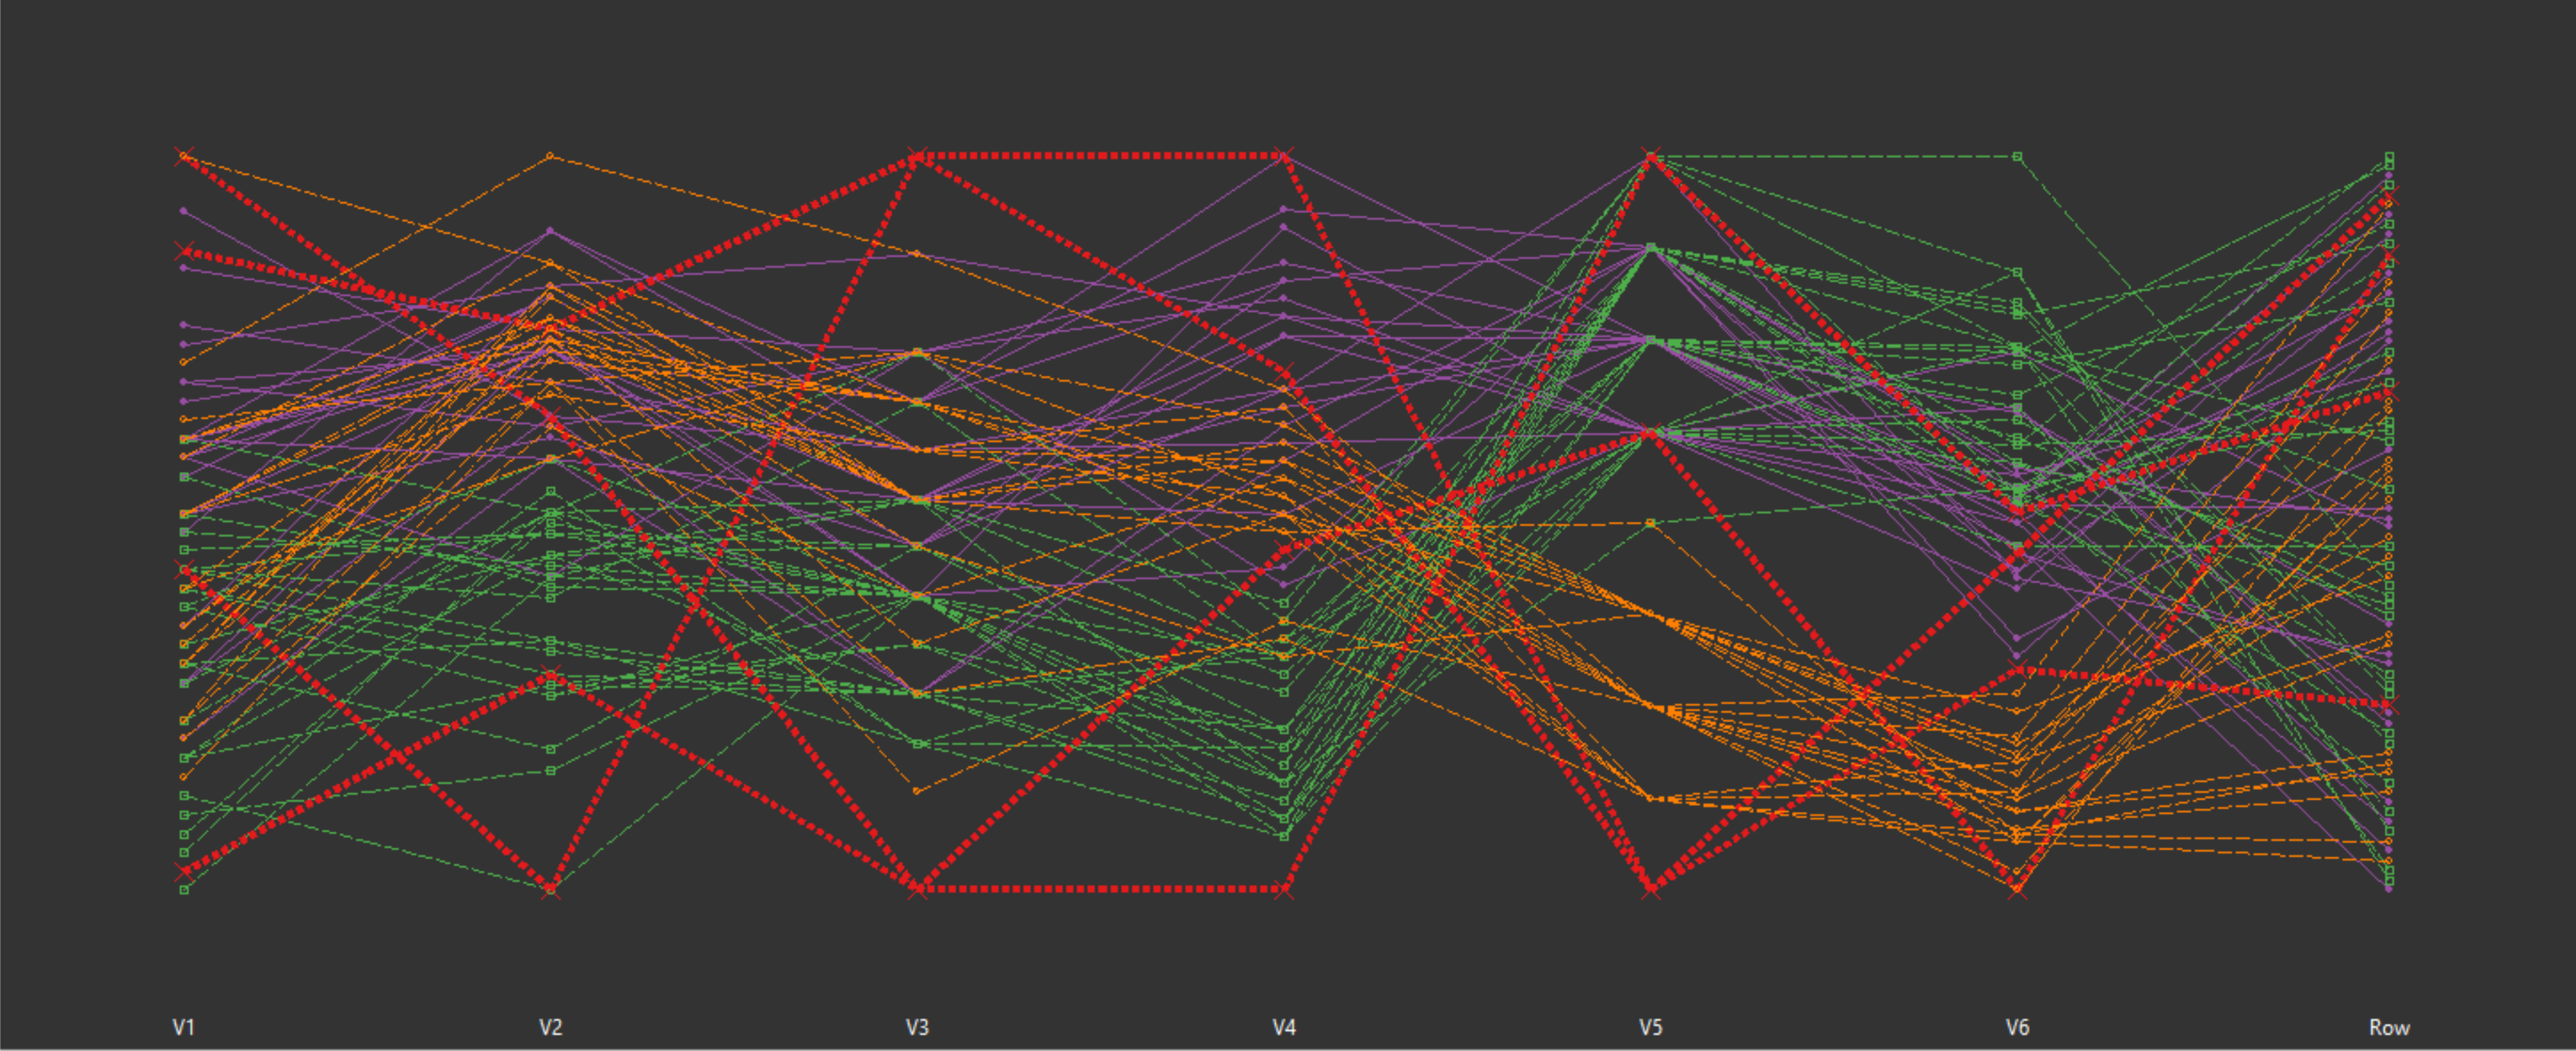
\includegraphics[width=11 cm]{p4c_PCP.png}\\
    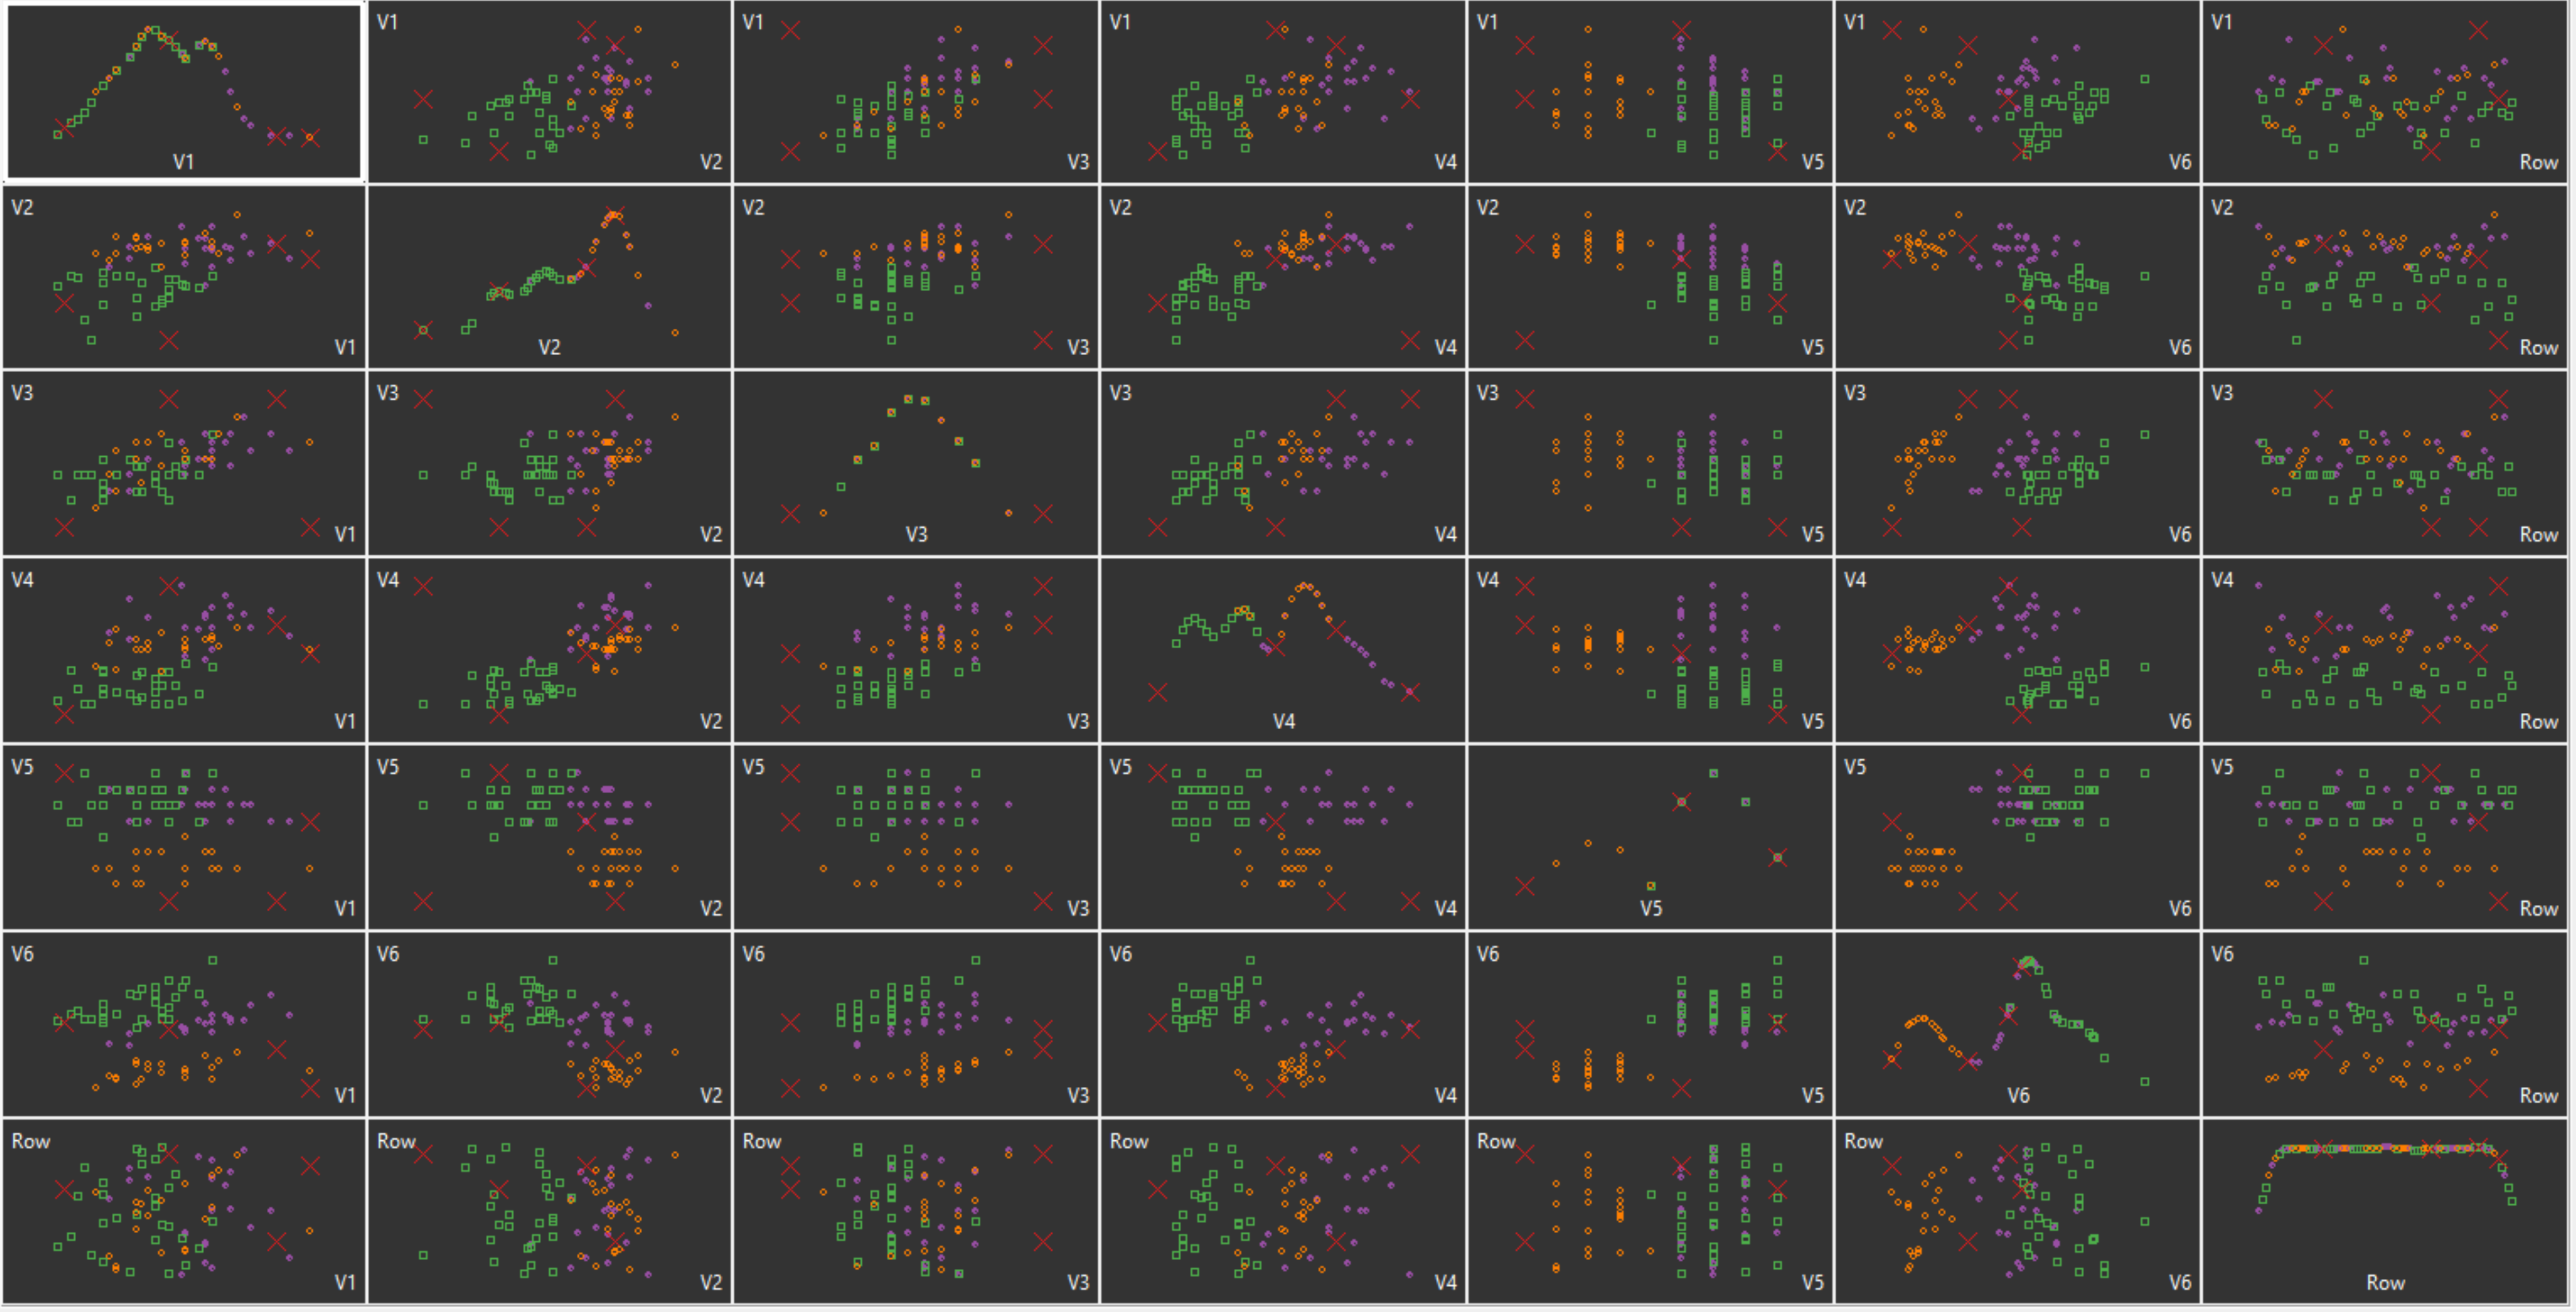
\includegraphics[width=11 cm]{p4c_scatter.png}\\
  \end{center}



\item (4 Points)
Revisit your outliers: What are the {\it Row} numbers for your outliers?
Note that {\it Identify} in {\it GGobi} provides you with the case number 
(or row label used by {\it GGobi}).
The {\it Row} number in our data set is the {\it GGobi} case number $+ 1$.
This becomes obvious in {\it Tools $\rightarrow$ Data Viewer}. 

Are you surprised how your outliers look in the PCP and the scatterplot matrix?
I would be $\ldots$ Is there a single axis in the PCP that would have
allowed you to detect a specific outlier (which outlier and which axis)? 
Is there any pairwise scatterplot in the scatterplot matrix that would have
allowed you to detect a specific outlier (which outlier and which pairwise scatterplot)? 
Using the variable axes information from the grand tour may help.

Verbally describe the characteristics of the outliers you detected. 

{\scriptsize
  The row number for the outliers I identified are {\bf 20, 52, 66,} and {\bf 72}.  In looking at the PCP and the scatterplot matrix, I was a little surprised (even given our earlier observations) that they were all easily identifiable on {\it V3} as either the highest or the lowest values.  This is true for all of the outliers in both the PCP and the scatterplot matrix.\\
  
  General characteristics of the outliers is there tendancy to bounce all over the PCP compaired to the tendancies of the clusters that were identified, that is to say that they ignore the overall behavior of the data.  In the scatterplot matrix however, it is much more difficult to identify general trends outside of {\it V3}.  In fact, I would go so far as to say that if I didn't already believe they were outliers from other visualizations, I would have had not likely been able to pick them out from just the scatterplot matrix.

}


\item (4 Points)
Revisit your clusters: How many did you detect visually?
Are there any variables in the PCP that would have allowed you
to identify the same clusters? Which ones? Is this a clear separation?

Are there any pairwise scatterplots in the scatterplot matrix that would have
allowed you to detect the same clusters? Which ones? Is this a clear separation?
When you refer to your clusters, identify them by the colors and glyphs
you used, e.g., the cluster made up by the ``yellow o'' and the cluster 
made up by the ``purple $+$''. 

{\scriptsize
  I visually detected three clusters, and viewing the PCP, I believe that examining {\it V5} and {\it V6} I would have been able to identify the {\color{orange} orange o} group as distinct. Then, I might have been able to further identify the {\color{green} green $\square$} by noting the pattern between {\it V4} and {\it V5}, and gaining evidence of this after examining {\it V2}.

There are only 2 plots in my scatterplot matrix that might allow me to have identified the three clusters they were {\it V4-V5} and {\it V4-V6}, and even then the seperation is relatively minamal, and thus difficult to identify.
}


\item (4 Points)
Overall, did we benefit from the grand tour, or could we just have used
a PCP and/or a scatterplot matrix? Be specific and justify your answer.
Compare which variable axes had most impact in the screenshots (or photos) you created
from the grand tour with subsets of these variables in the PCP and in the
pairwise scatterplots. 

{\scriptsize
  I believe that we benefited considerably from the use of the Grand Tour.  It allowed us the ability to patterns quickly, and with less ambiguity.  While I believe that it is definitely possible to identify these patterns in the PCP and the Scatterplot Matrix, the Grand Tour made for much quicker exploritory data analysis.  Then, viewing the PCP and the Scatterplot matrix served to confirm those initial observations.\\
  
  Compairing the Variable axes in the Grand Tour, the PCP and the Scatterplot matrix, it appear that {\it V3}, {\it V4}, {\it V5}, and {\it V6} had the most impact on the the subsetting of the data as I have identified it.\\
}

\end{enumerate}


\end{enumerate}


\newpage


\noindent{\Large \bf General Instructions}~\\


\begin{enumerate}
\item Create a single pdf document, using R Markdown, Sweave, or knitr.
When you take this course at the 6000--level, you have to use \LaTeX\ in
combination with Sweave or knitr.
You only have to submit this one document.

\item Include a title page that contains your name, your A--number, the number of
the assignment, the submission date, and any other relevant information.

\item Start your answers to each main question on a new page (continuing with the next
part of a question on the same page is fine). 
Clearly label each question and question part.

\item Show your R code for each question part!

\item Before you submit your homework, check that you
follow all recommendations from Google's R Style Guide
(see \url{https://google.github.io/styleguide/Rguide.xml}). 
Moreover, make sure that your R code is consistent, i.e., that you use the same
type of assignments and the same type of quotes throughout your entire homework.

\item Give credit to external sources, such as stackoverflow or help pages. Be specific
and include the full URL where you found the help (or from which help page you got 
the information). Consider R code from such sources as ``legacy code or third--party code'' 
that does not have to be adjusted to Google's R Style (even though it would be nice,
in particular if you only used a brief code segment).

\item {\bf Not following the general instructions outlined above will result in point deductions!}

\item For general questions related to this homework, please
use the corresponding discussion board in Canvas! I will try to
reply as quickly as possible. Moreover, if one of you knows
an answer, please post it. It is fine to refer to web pages
and R commands, but do not provide the exact R command with all required arguments
or which of the suggestions from a stackoverflow web page eventually worked for you! 
This will be the task for each individual student!

\item Submit your single pdf file via Canvas by the submission deadline.
Late submissions will result in point deductions as outlined on the syllabus.

\end{enumerate}


\end{document}

